\chapter{Representar quantidades}
\markboth{Módulo 1}{}

\section{Habilidades do SAEB}

\begin{itemize}
\item Escrever números racionais (naturais de até 6 ordens, representação
fracionária ou decimal finita até a ordem dos milésimos) em sua
representação por algarismos ou em língua materna ou associar o registro
numérico ao registro em língua materna.
\item Identificar a ordem ocupada por um algarismo ou seu valor posicional
(ou valor relativo) em um número natural de até 6 ordens.
\item Comparar ou ordenar números racionais (naturais de até 6 ordens,
representação fracionária ou decimal finita até a ordem dos milésimos),
com ou sem suporte da reta numérica.
\item Compor ou decompor números naturais de até 6 ordens na forma aditiva,
ou em suas ordens, ou em adições e multiplicações.
\item Comparar diferentes sentenças de adições ou de subtrações de dois
números naturais.
\item Determinar o número desconhecido que torna verdadeira uma igualdade
que envolve as operações fundamentais com números naturais de até 6
ordens.
\end{itemize}

\subsection{Habilidades da BNCC}

\begin{itemize}
\item EF04MA01, EF04MA02.
\end{itemize}

\conteudo{

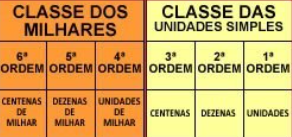
\includegraphics[width=\textwidth]{media/image1.png}\bigskip

Valor posicional ou relativo: é o valor que o algarismo assume
dependendo da classe e da ordem em que ele está posicionado no número.

Exemplo: no número 352.146, o algarismo 5 apresenta valor posicional ou
relativo igual a 50.000, pois ocupa a 5º ordem, a qual está dentro da
classe dos milhares; ou seja, está na posição da dezena de milhar e,
sendo assim, 5 x 10.000 = 50.000.

Sistema de numeração Egípcio: era baseado em figuras; cada figura tinha um valor específico e a combinação entre figuras formava as qantidades e os valores que se desejava representar. \bigskip

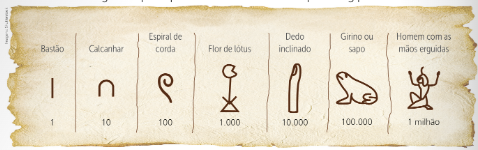
\includegraphics[width=\textwidth]{media/image2.png}\bigskip

\pagebreak
Sistema de numeração Maia: era baseado em representar
números com pontos e traços, conforme a figura.\bigskip

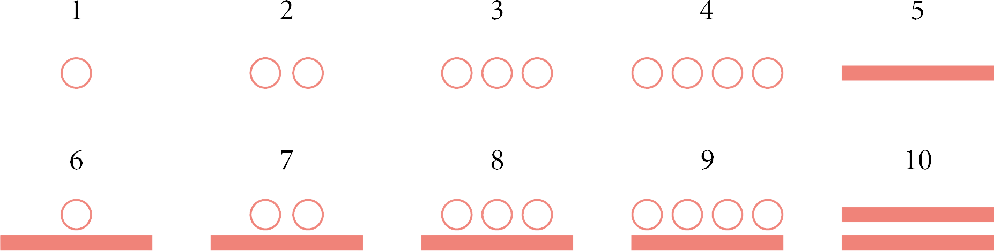
\includegraphics[width=\textwidth]{media/image3.png}\bigskip

Sistema de numeração Romano: representava os números com letras
maiúsculas, seguindo regras específicas para essa representação.\bigskip

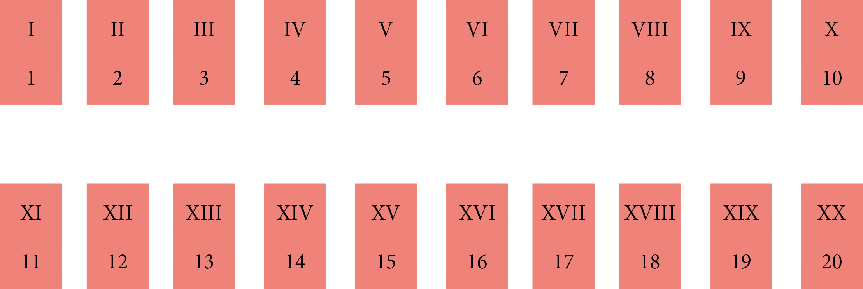
\includegraphics[width=\textwidth]{media/image4.png}\bigskip

Sistema de numeração indo-arábico: é o utilizado por nós
até hoje e, com o passar do tempo, foi evoluindo na escrita dos algarismos e, consequentemente, dos números, como está representado na figura.\smallskip

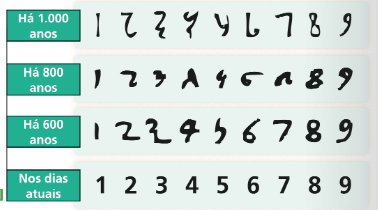
\includegraphics[width=.8\textwidth]{media/image5.png}
}

\section{Atividades}

\num{1} Escreva o valor posicional de cada algarismo
destacado -- ou seja, o valor que cada um assume de acordo com a posição
que ocupa no número.

\begin{escolha}
\item \textbf{8}24.345: \reduline{Valor posicional do 8 nesse caso: 800.000 -- centena de milhar.\hfill}

\item 3\textbf{7}5.6\textbf{7}8: \reduline{Valor posicional da primeira ocorrência do 7 nesse caso: 70.000 -- dezena de milhar. Valor posicional da segunda ocorrência do 7 nesse caso: 70 -- dezena comum.\hfill}

\item 14\textbf{8}.52\textbf{1}:
  \reduline{Valor posicional do 8 nesse caso: 8.000 -- unidade de milhar.\hfill}
  \reduline{Valor posicional do 1 nesse caso: 1 -- unidade comum.\hfill}
\end{escolha}

\num{2} Decomponha os números a seguir de acordo com o valor posicional de cada
algarismo.

\begin{escolha}
\item 32.084

\reduline{30 000 + 2 000 + 80 + 4; 3 x 10 000 + 2 x 1 000 + 0 x 100 + 8 x 10 + 4.\hfill}

\item
  26.587

\reduline{20 000 + 6 000 + 500 + 80 + 7; 2 x 10 000 + 6 x 1 000 + 5 x 100 + 8 x 10 + 7.\hfill}
  
\item
  2.105

\reduline{2 000 + 100 + 5; 2 x 1 000 + 1 x 100 + 0 x 10 + 5\hfill}
\end{escolha}


\num{3} Monte os número compostos e registre-os nas linhas a seguir.

\begin{escolha}
\item
  7 unidades de milhar, 5 centenas e 4 unidades: \reduline{7.504.\hfill}

\item
  3 dezenas de milhar, 7 dezenas e 2 unidades: \reduline{30.072.\hfill}

\item
  9 centenas de milhar, 5 unidades de milhar e 6 centenas: \reduline{905.600.\hfill}

\item
  2 unidades de milhar, 6 centenas e 3 unidades: \reduline{2.603\hfill}
\end{escolha}

%\coment{É necessário explorar bem a montagem dos números, pois muitos alunos sabem fazer a decomposição, mas não compreendem a volta.}

\num{4} Ligue um número da coluna da esquerda com a forma escrita correspondente na coluna da direita.

\begin{figure}[htpb!]
\centering
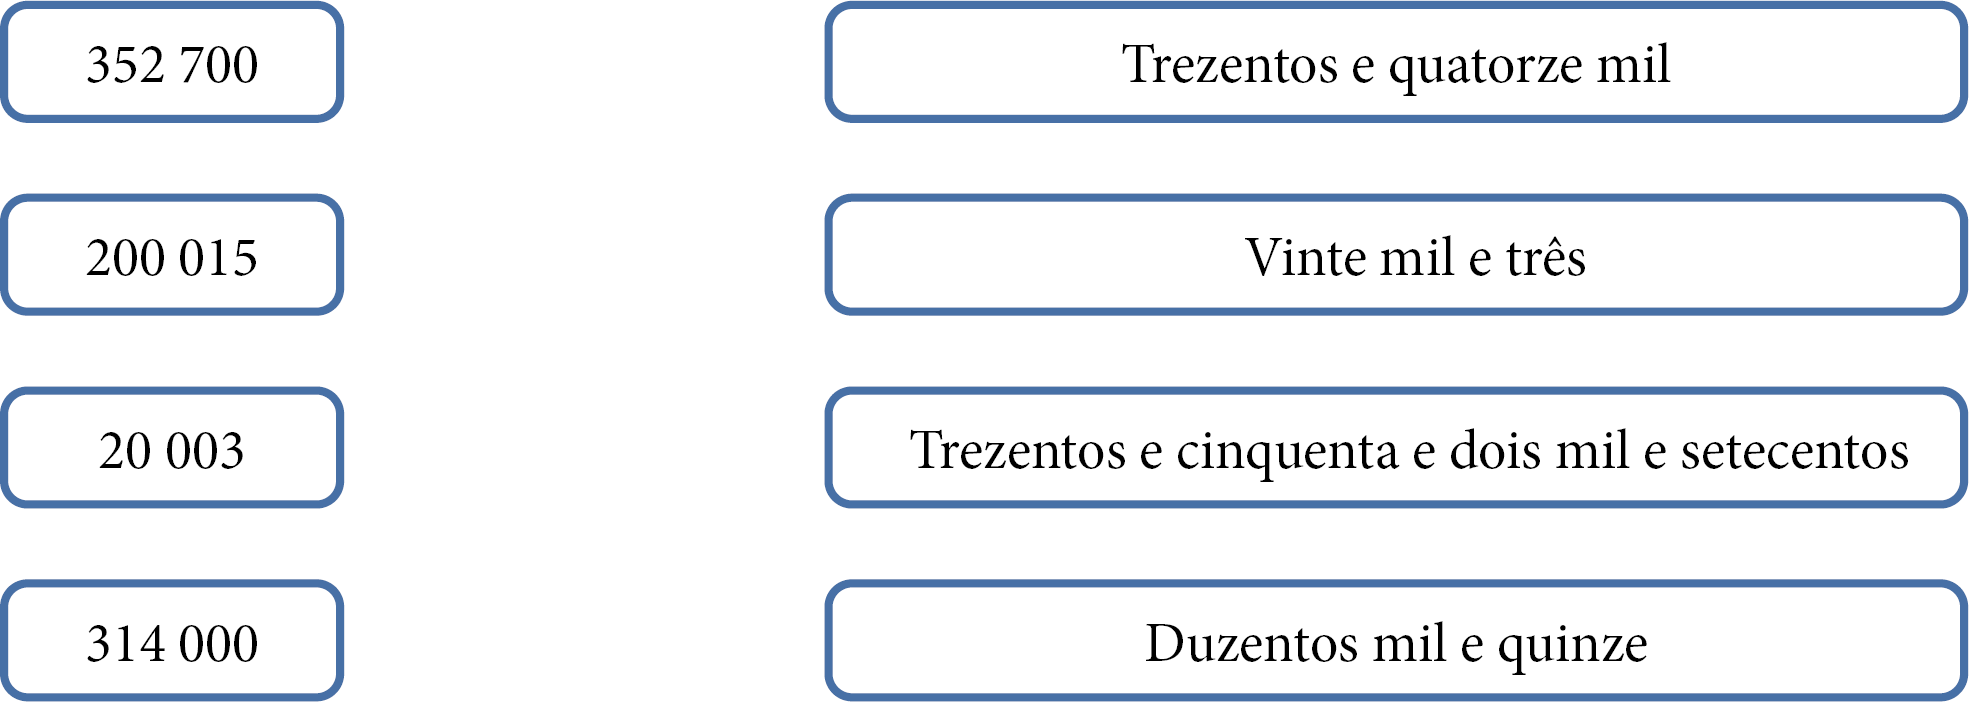
\includegraphics[width=\textwidth]{media/image6.png}
\end{figure}

%Resposta:
%352 700 deve estar ligado ao trezentos e cinquenta e dois mil e setecentos. 200 015 deve estar ligado ao duzentos mil e quinze. 20 003 deve estar ligado a vinte mil e três. 314 000 deve estar ligado ao trezentos e quatorze mil.

\num{5} Monte um número a partir de cada composição a seguir e escreva-o por extenso.

\begin{escolha}
\item 5 x 100 + 4 x 10 + 5 x 1 \reduline{545.\hfill}

\item 3 x 1.000 + 0 x 100 + 9 x 10 + 3 x 1 \reduline{3.093.\hfill}

\item 4 x 10.000 + 8 x 1.000 + 5 x 100 + 0 x 10 + 2 x 1 \reduline{48.502.\hfill}

\item 3 x 100.000 + 1 x 10.000 + 6 x 1.000 + 2 x 100 + 1 x 10 + 3 x 1 \reduline{316.213.\hfill}
\end{escolha}

\num{6} Escreva por extenso cada um dos números montados na atividade anterior.

\reduline{Quinhentos e quarenta e cinco.\hfill}

\reduline{Três mil e noventa e três.\hfill}

\reduline{Quarenta e oito mil quinhentos e dois.\hfill}

\reduline{Trezentos e dezesseis mil duzentos e treze.\hfill}

\pagebreak
\num{7} Observe os números no quadro a seguir e relacione cada um a uma característica.

\begin{mdframed}[linewidth=2pt,linecolor=azul!20,backgroundcolor=azul!20,roundcorner=2pt]
147.254 \hfill 464.823 \hfill 9.998 \hfill 99.999
\end{mdframed}

\begin{escolha}
\item O maior número com exatamente 5 ordens. \reduline{99.999.\hfill}

\item O segundo maior número formado por 4 ordens. \reduline{9.998.\hfill}

\item Um número ímpar com 6 ordens. \reduline{464 823.\hfill}

\item Um número de 6 ordens com algarismo da unidade de milhar igual a 7. \reduline{147.254.\hfill}
\end{escolha}

\num{8} Represente os números a seguir utilizando os símbolos maias.

\begin{escolha}
\item
  11

\begin{mdframed}[linewidth=2pt,linecolor=salmao,roundcorner=2pt]
\coment{O aluno deve usar duas linhas e um ponto.}
\vspace{1cm}
\end{mdframed}

\item
  12

\begin{mdframed}[linewidth=2pt,linecolor=salmao,roundcorner=2pt]
\coment{O aluno deve usar duas linhas e dois pontos.}
\vspace{1cm}
\end{mdframed}

\pagebreak
\item
  13

\begin{mdframed}[linewidth=2pt,linecolor=salmao,roundcorner=2pt]
\coment{O aluno deve usar duas linhas e três pontos.}
\vspace{1cm}
\end{mdframed}

\item
  14

\begin{mdframed}[linewidth=2pt,linecolor=salmao,roundcorner=2pt]
\coment{O aluno deve usar duas linhas e quatro pontos.}
\vspace{1cm}
\end{mdframed}

\item
  15

\begin{mdframed}[linewidth=2pt,linecolor=salmao,roundcorner=2pt]
\coment{O aluno deve usar duas linhas seguidas de uma linha.}
\vspace{1cm}
\end{mdframed}

\item
  16

\begin{mdframed}[linewidth=2pt,linecolor=salmao,roundcorner=2pt]
\coment{O aluno deve usar duas linhas seguidas de um ponto sobre uma linha.}
\vspace{1cm}
\end{mdframed}

\item
  17

\begin{mdframed}[linewidth=2pt,linecolor=salmao,roundcorner=2pt]
\coment{O aluno deve usar duas linhas seguidas de dois pontos sobre uma linha.}
\vspace{.5cm}
\end{mdframed}

\pagebreak
\item
  18

\begin{mdframed}[linewidth=2pt,linecolor=salmao,roundcorner=2pt]
\coment{O aluno deve usar duas linhas seguidas de três pontos sobre uma linha.}
\vspace{1cm}
\end{mdframed}

\item
  19

\begin{mdframed}[linewidth=2pt,linecolor=salmao,roundcorner=2pt]
\coment{O aluno deve usar duas linhas seguidas de quatro pontos sobre uma linha.}
\vspace{1cm}
\end{mdframed}

\end{escolha}

\num{9} Escreva cada um dos números a seguir utilizando o sistema indo-arábico.

\begin{escolha}
\item
  Dois mil trezentos e cinco: \reduline{2.305\hfill}
\item
  Quinze mil e quarenta e sete: \reduline{15.047\hfill}
\item
  Vinte mil e novecentos: \reduline{20.900\hfill}
\item
  Trinta e três mil trezentos e trinta e três: \reduline{33.333\hfill}
\item
  Cinquenta mil e cinco: \reduline{50.005\hfill}
\end{escolha}

\pagebreak
\num{10} A bolas representadas a seguir fazem parte de um jogo conhecido como
bilhar ou como sinuca.

\begin{figure}[htpb!]
\centering
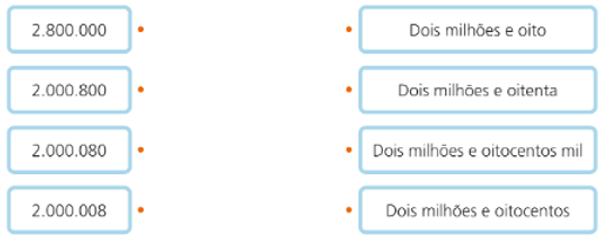
\includegraphics[width=\textwidth]{media/image7.png}
\end{figure}


Observando os números representados em cada bola, responda ao que se pergunta a seguir.

\begin{escolha}
\item
  Qual é o menor número entre essas bolas? \reduline{2 (dois).\hfill}

\item
  Qual é o menor número com exatamente 4 ordens que podemos formar com essas bolas? \reduline{2.789 (dois mil setecentos e oitenta e nove).\hfill}

\item
  Qual é o maior número par que podemos formar com essas bolas? \reduline{9.872 (nove mil oitocentos e setenta e dois).\hfill}
\end{escolha}

%Explore mais exemplos com os alunos para estimular a formação de números e a criatividade de cada um deles.

\section{Treino}

\num{1} Amanda estava brincando no escritório de seu pai quando encontrou um
pedaço de papel em que estava escrito isto:

\begin{figure}[htpb!]
\centering
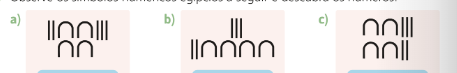
\includegraphics[width=.4\textwidth]{media/image8.png}
\end{figure}

\pagebreak
Lembrando-se das aulas de Matemática, a menina resolveu decompor o número escrito
no papel. Qual é a decomposição correta que Amanda poderá fazer desse
número?

\begin{escolha}
\item
  600.000 + 50.000 + 700 + 30 + 4.
\item
  600.000 + 5.000 + 70 + 3 + 4.
\item
  600.000 + 500 + 700 + 30 + 4.
\item
  60.000 + 50.000 + 70 + 300 + 4.
\end{escolha}

\num{2} Vitor escreveu o seguinte número utilizando os algarismos romanos:

\begin{myquote}
XIX
\end{myquote}

Esse número, no sistema indo-arábico, é o:

\begin{escolha}
\item
  9.
\item
  19.
\item
  21.
\item
  11.
\end{escolha}

\pagebreak
\num{3} José resolveu comprar uma placa com o número de sua casa. Observe a seguir.

\begin{figure}[htpb!]
\centering
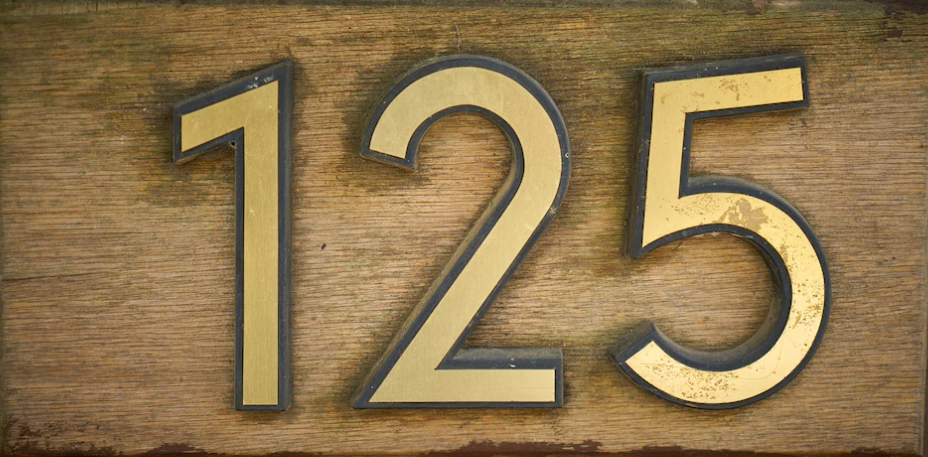
\includegraphics[width=\textwidth]{media/image9.png}
\end{figure}

Depois, percebeu que o número estava
errado, já que o primeiro e o último algarismo estão nas posições
trocadas. Qual é o valor relativo do último algarismo no lugar em que ele se
encontra na placa errada e qual deveria ser seu valor relativo no número
correto da casa de José?

\begin{escolha}
\item
  Está como 5 e deveria ser como 50.
\item
  Está como 50 e deveria ser como 500.
\item
  Está como 5 e deveria ser como 500.
\item
  Está como 50 e deveria ser como 5.
\end{escolha}

\chapter{As operações básicas}
\markboth{Módulo 2}{}

\section{Habilidades do SAEB}

\begin{itemize}
\item Calcular o resultado de adições ou subtrações envolvendo números
naturais de até 6 ordens.
\item Calcular o resultado de multiplicações ou divisões envolvendo números
naturais de até 6 ordens.
\item Associar o quociente de uma divisão com resto zero de um número
natural de até 6 ordens por 2, 3, 4, 5 e 10 às ideias de metade, terça,
quarta, quinta e décima parte.
\item Resolver problemas de adição ou de subtração, envolvendo números
naturais de até 6 ordens, com os significados de juntar, acrescentar,
separar, retirar, comparar ou completar.
\item Resolver problemas de multiplicação ou de divisão, envolvendo números
naturais de até 6ordens, com os significados de formação de grupos
iguais (incluindo repartição equitativa e medida), proporcionalidade ou
disposição retangular.
\end{itemize}

\subsection{Habilidade da BNCC}

\begin{itemize}
\item EF04MA07.
\end{itemize}

\conteudo{
\begin{itemize}
\item\textbf{Adição}
\end{itemize}


\includegraphics[width=.3\textwidth]{media/image10.png}

\pagebreak
\begin{itemize}
\item\textbf{Subtração}
\end{itemize}

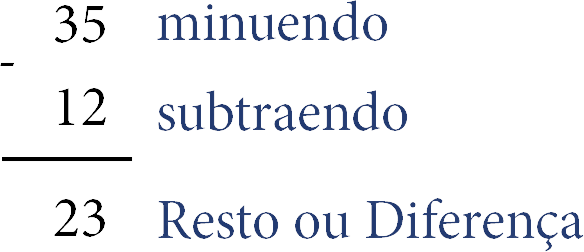
\includegraphics[width=.3\textwidth]{media/image11.png}

\begin{itemize}
\item\textbf{Multiplicação}
\end{itemize}

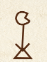
\includegraphics[width=.3\textwidth]{media/image12.png}

\begin{itemize}
\item\textbf{Divisão}
\end{itemize}

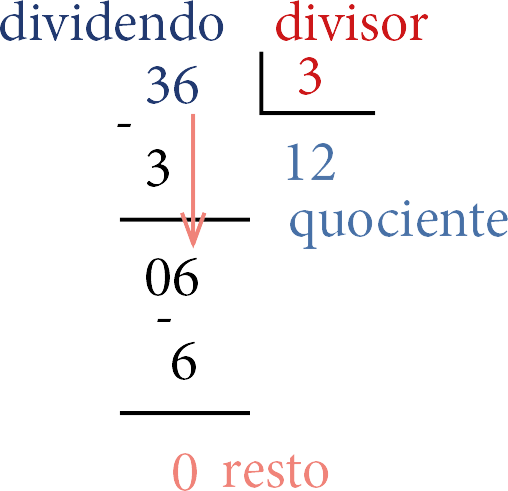
\includegraphics[width=.3\textwidth]{media/image13.png}
}

\pagebreak
\section{Atividades}

\num{1} Ligue cada operação da coluna da esquerda com o resultado correto na
coluna da direita.

\begin{figure}[htpb!]
\centering
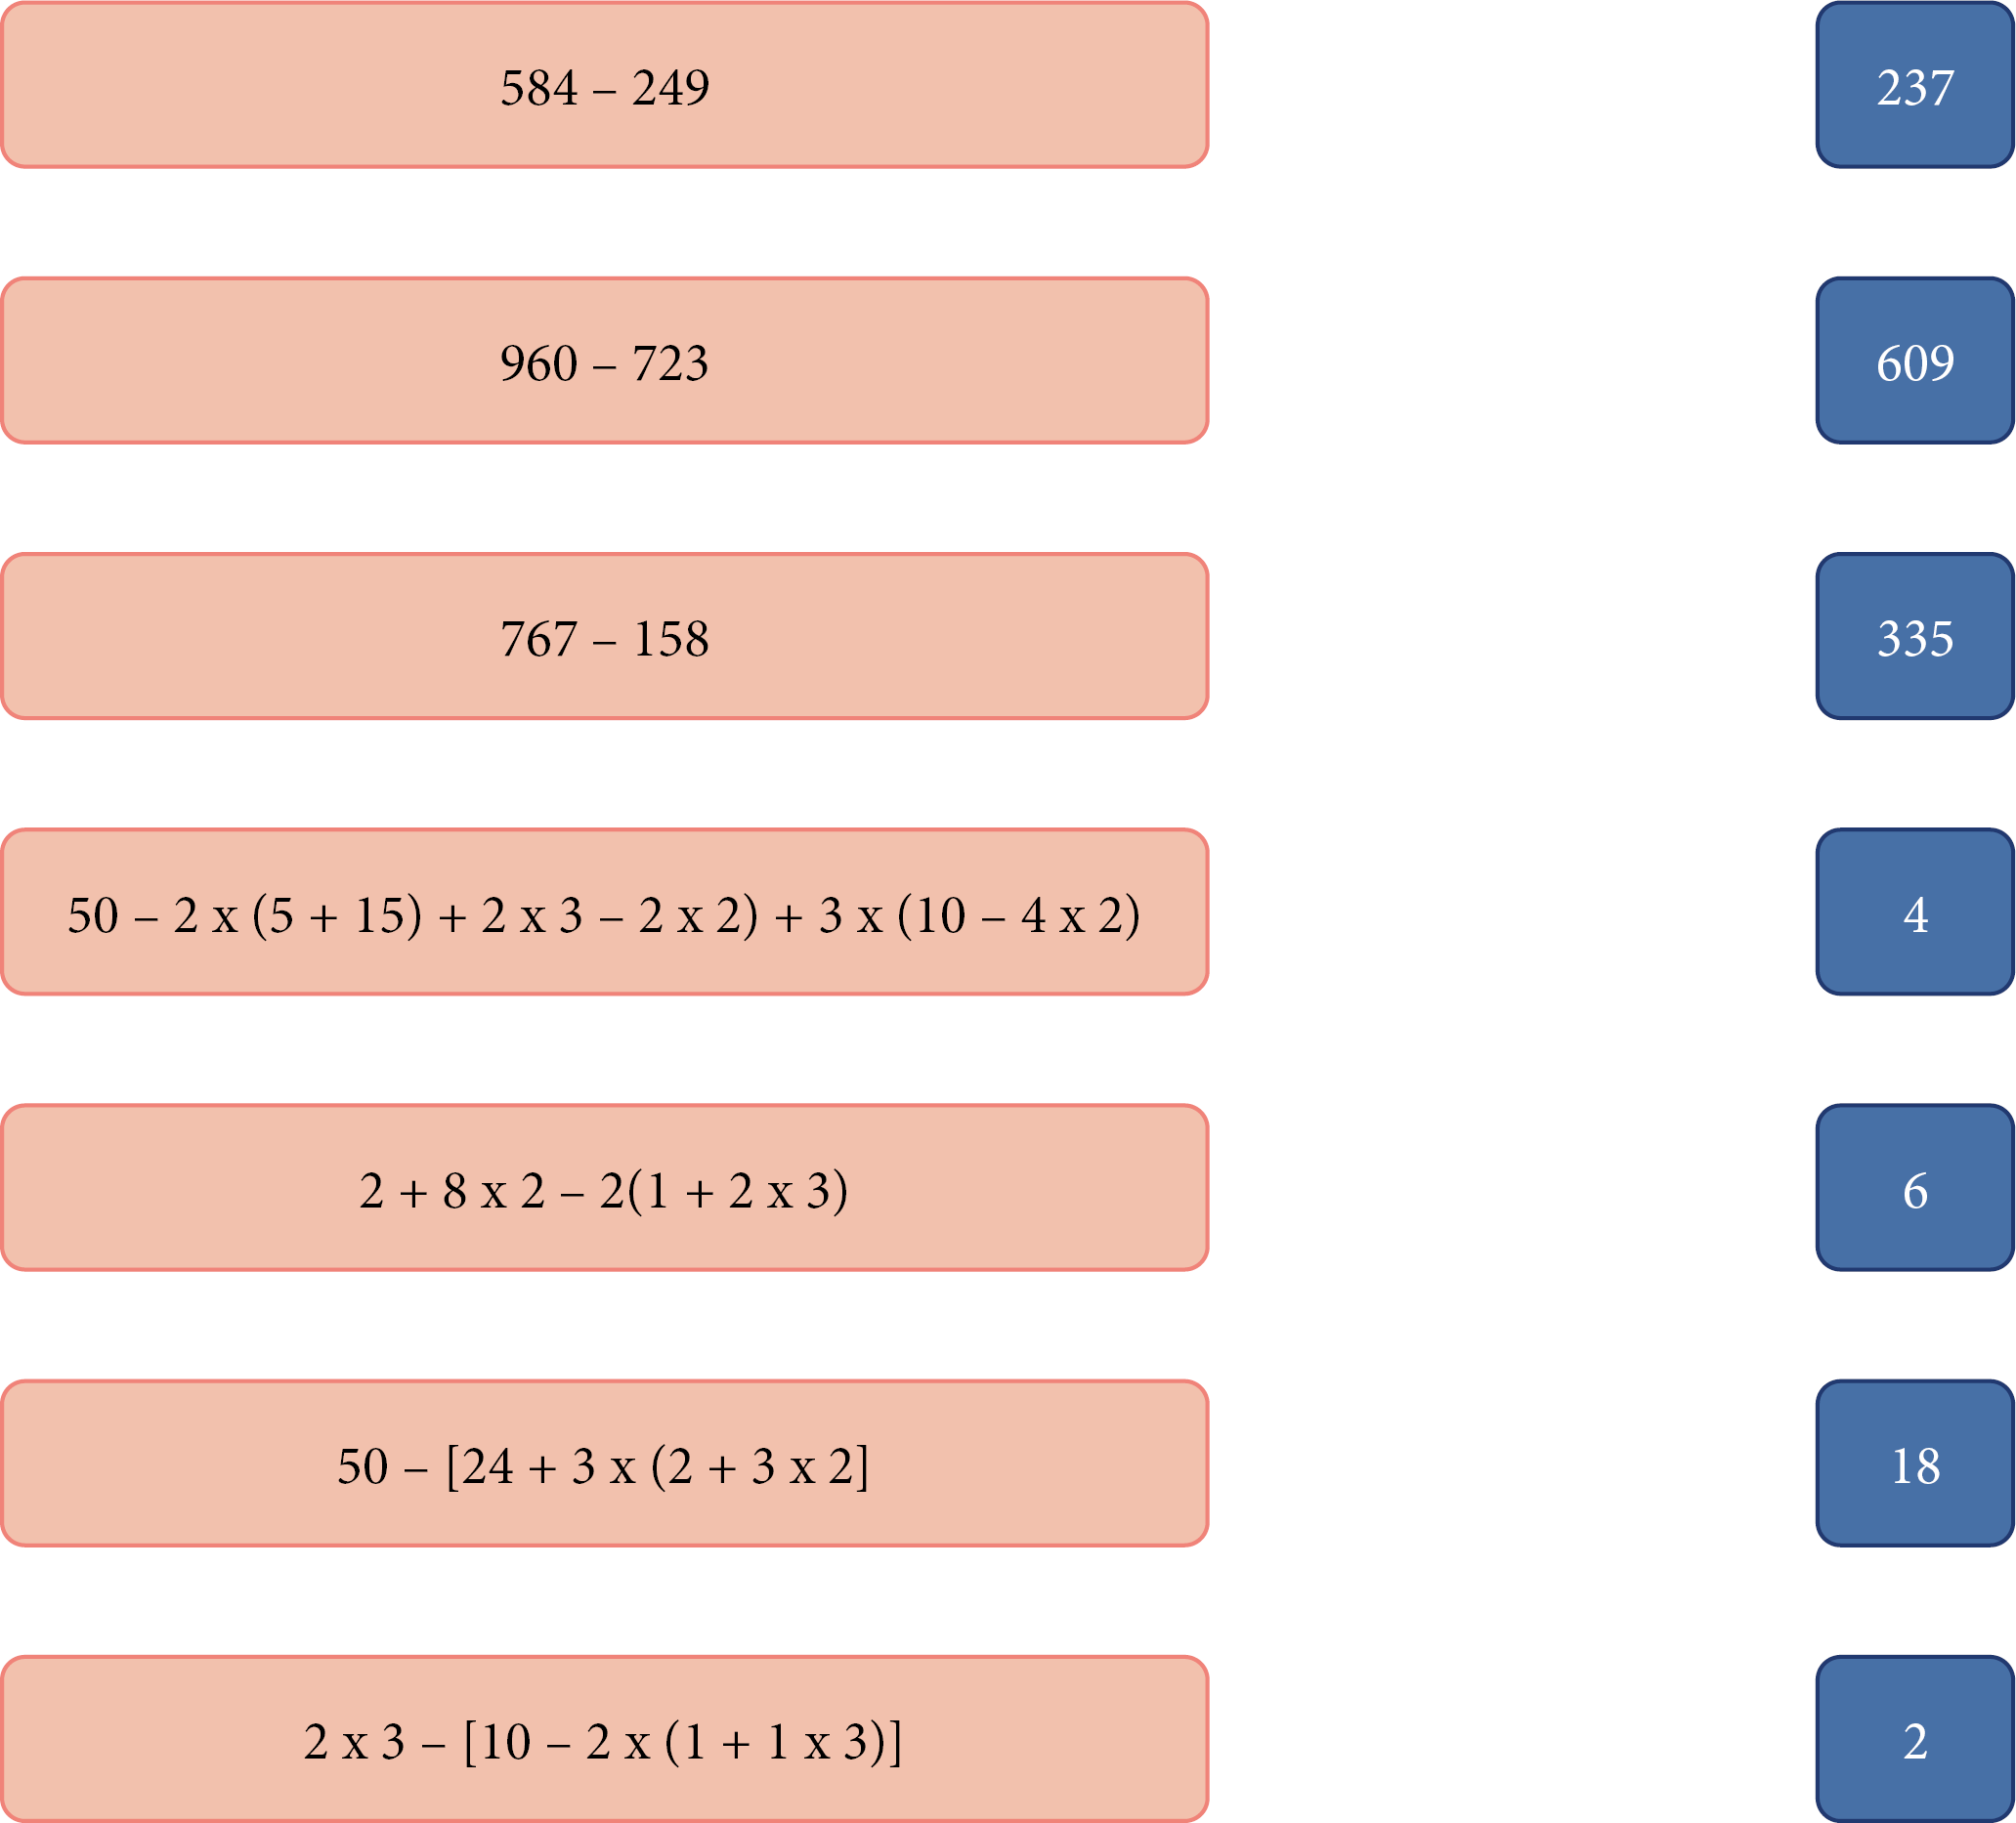
\includegraphics[width=\textwidth]{media/image14.png}
\end{figure}

\num{2} Segunda a receita de um bolo, devem-se inicialmente colocar 260 g de farinha
de trigo e misturar com outros ingredientes como ovos, açúcar e leite.
Em seguida, devem-se colocar mais 135 g de farinha de trigo para a massa
ficar no ponto ideal. Qual é a quantidade total de farinha, em quilogramas,
utilizada nessa receita?

\begin{mdframed}[linewidth=2pt,linecolor=salmao,roundcorner=2pt]
\coment{260 + 135 = 395 g = 0,395 kg}
\vspace{3cm}
\end{mdframed}

\num{3} A tabela a seguir mostra a população do Amapá dividida em municípios, segundo estimativa do IBGE de 2018.

\begin{longtable}[]{@{}ll@{}}
\toprule
Município & População estimada\tabularnewline
\midrule
\endhead
Macapá (capital) & 503.907\tabularnewline
Santana & 122.988\tabularnewline
Laranjal do Jari & 55.021\tabularnewline
Oiapoque & 29.563\tabularnewline
Mazagão & 27.436\tabularnewline
Porto Grande & 22.286\tabularnewline
Tartarugalzinho & 17.206\tabularnewline
Pedra Branca do Amapari & 16.624\tabularnewline
Vitória do Jari & 15.632\tabularnewline
Calçoene & 12.165\tabularnewline
Amapá & 10.842\tabularnewline
Ferreira Gomes & 9.373\tabularnewline
Cutias & 7.816\tabularnewline
Itaubal & 6.400\tabularnewline
Serra do Navio & 6.301\tabularnewline
Pracuuba & 5.632\tabularnewline
\bottomrule
\end{longtable}

A somatória das populações dos municípios sem contar a capital é maior ou menor que a população de Macapá? Justifique sua resposta com cálculos.

\begin{mdframed}[linewidth=2pt,linecolor=salmao,roundcorner=2pt]
\coment{122.988 + 55.021 + 29.563 + 27.436 + 22.286 + 17.206 + 16.624 + 15.632 + 12.165 + 10.842 + 9.373 + 7.816 + 6.400 + 6.301 + 5.632 = 365.285 (menor que a população da capital, que é de 503.907).}

\coment{Portanto a soma das populações estimadas dos municípios apresentados na
tabela, exceto São Paulo, é menor que a população da cidade de São
Paulo.}
\end{mdframed}

\num{4} Faça o que se pede a seguir.

\begin{escolha}
\item
  Se em uma caixa cabem 1.000 bolinhas de gude de mesmo tamanho, quantas
  caixas precisaremos para guardar 6.536 bolinhas de gude desse mesmo
  tamanho?

\reduline{6.536 : 1.000 = 6 + 536 de resto; portanto serão necessárias 7 caixas
    (6 caixas completas e 1 com 536 bolinhas apenas).\hfill}

\item
  Se na caixa couberem apenas 100 bolinhas de gude de mesmo tamanho, quantas
  caixas serão necessárias para armazenar essas mesmas 6.536 bolinhas?

\reduline{6.536 : 100 = 65 + 36 de resto; portanto serão necessárias 66 caixas
    (65 caixas completas e 1 com 36 bolinhas apenas).\hfill}

\item
  Se a caixa só puder armazenar 10 bolinhas de mesmo tamanho, quantas caixas dessas
  serão necessárias para armazenar as mesmas 6.536 bolinhas de gude?

\reduline{6.536 : 10 = 653 + 6 de resto; portanto serão necessárias 654 caixas
    (653 caixas completas e 1 com 6 bolinhas apenas).\hfill}
\end{escolha}

\pagebreak
\num{5} Faça o que se pede a seguir.

\begin{escolha}
\item Uma coleção de álbum de figurinhas conta com cinco volumes temáticos: animais da savana, animais da Ásia, animais da Austrália, animais do Ártico e animais das Américas. Em cada volume, a pessoa precisa de 45 figurinhas para completar o álbum. Calcule quantas figurinhas são necessárias para completar a coleção toda.

\reduline{São necessárias 45 figurinhase em cada volume, e são 5 volumes. Logo: 5 x 45 = 225 figurinhas para a coleção toda.\hfill}

\item Uma grande exposição de obras de arte de vários artistas está dividida em 108 seções, e em cada seção há entre 6 e 9 obras de arte. Calcule o número mínimo e o número máximo de obras que pode haver na exposição toda?

\reduline{Cada seção pode ter no mínimo 6 obras de arte. Logo: 108 x 6 = 648 obras de arte no mínimo na exposição toda. Cada seção pode ter no máximo 9 obras de arte. Logo: 108 x 9 = 972 obras de arte no máximo na exposição toda.\hfill}

\item Um estádio de futebol pequeno tem, na arquibancada superior, 66 fileiras de 302 assentos. Calcule a lotação máxima da arquibancada superior desse estádio.

\reduline{São 66 fileiras x 302 assentos = 19.932 assentos no total.\hfill}
\end{escolha}

\num{6} O pai de Marcela trabalha em uma transportadora e, em determinado
dia, seu caminhão foi carregado com 64 engradados de refrigerantes.
Em cada engradado, há 12 garrafas de refrigerante. Cada garrafa de refrigente
contém 2 litos.

\pagebreak
Quantos litros de refrigerante o pai de Marcela tinha em seu caminhão?

\begin{mdframed}[linewidth=2pt,linecolor=salmao,roundcorner=2pt]
\coment{64 x 12 x 2 = 1.536 litros de refrigerante.}
\vspace{2cm}
\end{mdframed}

\num{7}

\begin{minipage}{.5\textwidth}
João
possui uma distribuidora de ovos e acabou de receber 14 caixas com 310
ovos cada uma. Para que João venda essa mercadoria, ele faz embalagens
de 12 ovos. Quantas embalagens João conseguirá fazer para
colocar à venda os ovos que acabou de receber? Haverá alguma sobra?
\end{minipage}\hspace{.5cm}
\begin{minipage}{.5\textwidth}

\includegraphics[width=\textwidth]{media/image15.png}
\end{minipage}

\begin{mdframed}[linewidth=2pt,linecolor=salmao,roundcorner=2pt]
\coment{(14 x 310) : 12 = 361 embalagens com 12 ovos cada uma e uma sobra de 8
ovos.}

\coment{Professor sempre escreva a expressão formada pela interpretação do
enunciado, pois assim os alunos vão aprendendo a transformar textos em linguagem
matemática.}
\end{mdframed}

\num{8} O livro que Gabriel está lendo possui 12 capítulos com 22 páginas cada
um. Se ele ler 10 páginas por dia, em quantos dias ele terminará de ler
o livro?

\begin{mdframed}[linewidth=2pt,linecolor=salmao,roundcorner=2pt]
\coment{(12 x 22) : 10 = 26 dias lendo 10 páginas por dia e 1 dia lendo 4 páginas; portanto terminará o livro em 27 dias.}
\vspace{2cm}
\end{mdframed}

\num{9} O pai de Pedro propôs a ele um grande desafio:
o pai fornece uma conta com um número escondido e o filho 
descobre qual número está escondido. Ajude Pedro com esse desafio e
encontre o número que está escondido pelo ponto de interrogação.

\begin{figure}[htpb!]
\centering
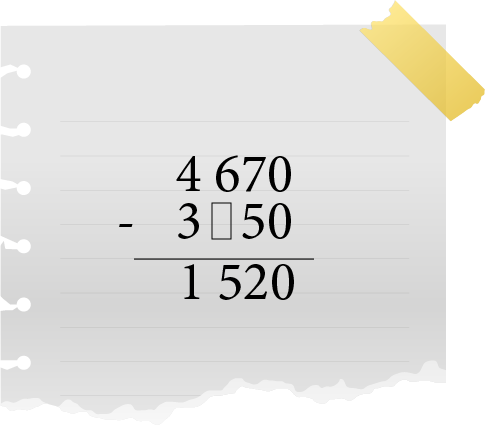
\includegraphics[width=.5\textwidth]{media/image16.png}
\end{figure}

\coment{O algarismo escondido é o 1.}

\num{10} Na fazendo do avô de Vinícius, há 104 galinhas, 62 porcos, 6 cavalos e 72
bois. Se na fazendo de seu vizinho o número de animais é o triplo do que
há na fazenda do avô, quantos animais estão presentes na fazenda do
vizinho?

\begin{mdframed}[linewidth=2pt,linecolor=salmao,roundcorner=2pt]
\coment{Número de animais na fazenda do avô: 104 + 62 + 6 + 72 = 244 animais.}

\coment{Número de animais na fazenda do vizinho: 244 x 3 = 732 animais.}
\vspace{1cm}
\end{mdframed}

\section{Treino}

\num{1} Verificando algumas atividades realizadas na escola no ano anterior,
Gustavo se deparou com uma conta em que 417 era o minuendo, mas o subtraendo
estava coberto por um retângulo. A diferença estava visível: 105.
Gustavo ficou curioso e resolveu refazer a atividade para descobrir o
número que faltava e, após alguns minutos, conseguiu descobrir. O número
que Gustavo encontrou é o

\begin{multicols}{2}
\begin{escolha}
\item
  128.
\item
  312.
\item
  158.
\item
  256.
\end{escolha}
\end{multicols}

\num{2} Isaac estava conferindo o estoque de mercadorias de sua loja e percebeu
que inicialmente ele tinha 200 peças. Depois vendeu 2 caixas com peças
para Carlos. Em cada uma das caixas havia um pacote com 5 unidades de peças e dois
pacotes com 7 peças. Para saber a quantidade de peças que restavam no estoque, Isaac fez a
seguinte anotação:

\begin{myquote}
200 -- 2 x (1 x 5 + 2 x 7)
\end{myquote}

O resultado dessa expressão era exatamente igual à quantidade de peças
que restavam em seu estoque após a venda para Carlos. Qual é a
quantidade de peças que Isaac possui agora em seu estoque?

\begin{multicols}{2}
\begin{escolha}
\item
  72.
\item
  94.
\item
  126.
\item
  162.
\end{escolha}
\end{multicols}


\num{3} Um grande circo chegou à cidade em que Rafael mora, e logo uma fila
enorme se formou com pessoas querendo assistir ao espetáculo. Os
ingressos começaram a ser vendidos e as pessoas começaram a entrar no
recinto do circo. Em certo instante sabia-se que 540 pessoas já tinham
entrado e que a capacidade máxima por espetáculo nesse circo era de 1.200 pessoas. Ainda estão na fila 932 pessoas. Quantas pessoas não
conseguirão entrar para assistir a essa sessão do circo?

\begin{multicols}{2}
\begin{escolha}
\item
  268.
\item
  272.
\item
  294.
\item
  440.
\end{escolha}
\end{multicols}


\chapter{Sequências}
\markboth{Módulo 3}{}

\section{Habilidades do SAEB}

\begin{itemize}
\item Inferir ou descrever atributos ou propriedades comuns que os elementos
que constituem uma sequência recursiva de números naturais apresentam.

\item Inferir o padrão ou a regularidade de uma sequência de números
naturais ordenados, objetos ou figuras.

\item Inferir os elementos ausentes em uma sequência de números naturais
ordenados, objetos ou figuras.
\end{itemize}

\subsection{Habilidade da BNCC}

\begin{itemize}
\item EF04MA11.
\end{itemize}

\conteudo{
Uma sequência ou sucessão é um conjunto ordenado no qual
existe sempre uma lógica de formação. Veja exemplos a seguir.

\begin{itemize}
\item
  A escalação de um time de futebol de salão em ordem alfabética: Alan; Bruno; Fernando; Igor; Tácio.
\item
  A sequência de números naturais pares: (0; 2; 4; 6; 8; 10; 12; ...).
\end{itemize}

Podemos classificar as sequências quanto ao número de elementos:

\begin{itemize}
\item
  \textbf{Finitas}: apresentam um número de termos bem definido.
\item
  \textbf{Infinitas}: apresentam infinitos números de termos, como
  a sequência dos números naturais.
\end{itemize}

Ainda podemos classificar as sequências numéricas desta forma:

\begin{itemize}
\item
  \textbf{Crescentes}: aquelas em que cada termo sucessor é maior que seu
  antecessor. Exemplo: (5, 10, 15, 20, 25).
\item
  \textbf{Decrescentes}: aquelas em que cada termo sucessor é menor que
  seu antecessor. Exemplo: (9, 7, 5, 3).
\end{itemize}
}

\section{Atividades}

\num{1} Observe as sequências dadas e determine o oitavo termo.

\begin{escolha}
  \item (4; 7; 10; 13...) \reduline{(8 x 3) + 1 = 25\hfill}

  \item (3; 6; 9...) \reduline{8 x 3 = 24\hfill}

  \item (4; 8; 12...) \reduline{8 x 4 = 32\hfill}

  \item (5; 10; 15; 20...) \reduline{8 x 5 = 40\hfill}
  \end{escolha}

\num{2} Observe atentamente a sequência numérica que Robson construiu e depois
faça o que se pede.

\begin{figure}[htpb!]
\centering
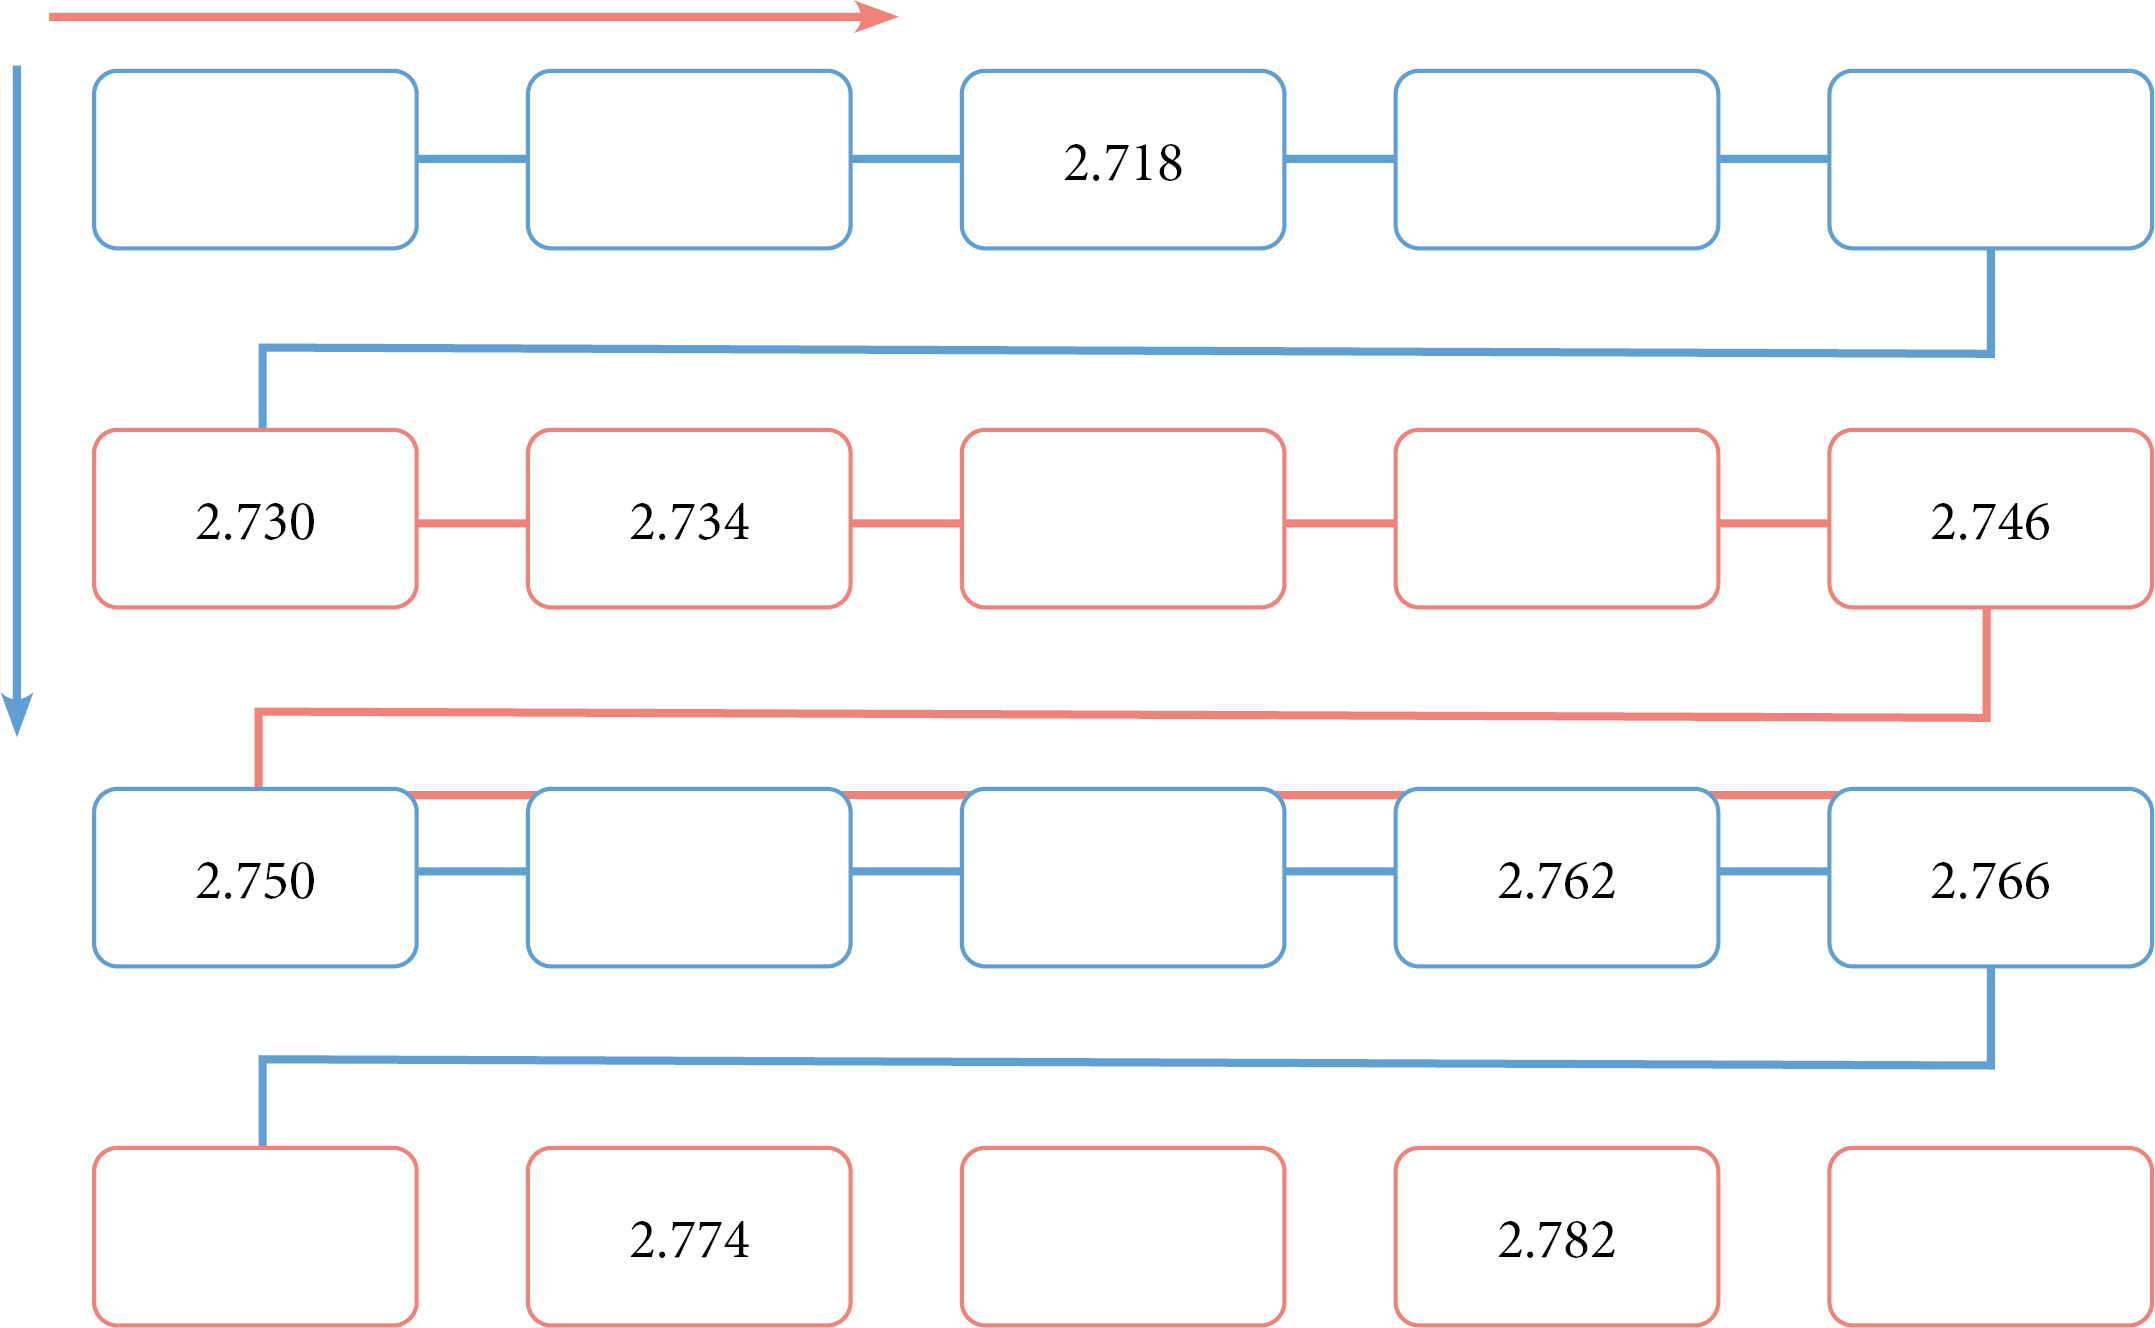
\includegraphics[width=.8\textwidth]{media/image17.png}
\end{figure}

\begin{escolha}
\item
  Qual lógica Robson utilizou para construir essa sequência?

\reduline{Em cada coluna, ele foi aumentando os números em 10 unidades, enquanto,
em cada linha, o aumento foi de 4 unidades. Outra forma de pensar é que, seguindo as setas colocadas
por ele, o aumento sempre foi de 4 unidades de um número para o próximo.
Professor explore as duas situações com os alunos.\hfill}

\item
  Complete a sequência com os números que estão faltando.

%\reduline{Linha 1: 2.710; 2.714; 2.718; 2.722; 2.726.\hfill}
%\reduline{Linha 2: 2.730; 2.734; 2.738; 2.742; 2.746.\hfill}
%\reduline{Linha 3: 2.750; 2.754; 2.758; 2.762; 2.766.\hfill}
%\reduline{Linha 4: 2.770; 2.774; 2.778. 2.782; 2.786.\hfill}
\end{escolha}

\num{3} Encontre o número pedido em cada item a seguir.

\begin{escolha}
\item
  O sucessor de 4.089: \reduline{4 090\hfill}

\item
  O antecessor de 5.301: \reduline{5 300\hfill}

\item
  O sucessor e o antecessor do número 4.259: \reduline{4.258 e 4.260\hfill}
\end{escolha}


\num{4} Entre os cadernos de seu irmão, Ana Clara encontrou um papel em que estava escrito assim: (231; 288; 245; 402; ...). Ela ficou muito curiosa, pois entendeu que essa era uma sequência
numérica, e queria encontrar o próximo número. Ajude Ana Clara a descobrir qual é o próximo número da sequência e o escreva no espaço a seguir.

\begin{mdframed}[linewidth=2pt,linecolor=salmao,roundcorner=2pt]
\coment{A sequência foi montada sempre somando-se 57 ao número anterior para
encontrar o próximo. Portanto o próximo número da sequência será: 402 +
57 = 459.}
\vspace{4.5cm}
\end{mdframed}

\pagebreak
\num{5} Organize os números a seguir em ordem decrescente.

\begin{figure}[htpb!]
\centering

\includegraphics[width=\textwidth]{media/image18.png}
\end{figure}

\begin{mdframed}[linewidth=2pt,linecolor=salmao,roundcorner=2pt]
\coment{Ordem decrescente (do maior para o menor):
11.111; 11.100; 11.010; 11.000; 10.111; 10.001; 1.111.}
\end{mdframed}

\num{6} O Pai de André montou a sequência de figuras a seguir.

\begin{figure}[htpb!]
\centering

\includegraphics[width=\textwidth]{media/image19.png}
\end{figure}

Em seguida, disse ao filho que o levaria ao cinema caso ele acertasse
qual seria o 20º termo dessa sequência. André, muito empolgado, começou a
pensar e logo deu a resposta a seu pai. O pai analisou a resposta e
disse que estava correta. Qual resposta André deu a seu pai sobre qual era o décimo elemento
dessa sequência?

\begin{mdframed}[linewidth=2pt,linecolor=salmao,roundcorner=2pt]
\coment{Só teremos triângulos em múltiplos de 3. Como 20 não é um
múltiplo de 3, a vigésima figura será um quadrado.}

\coment{É possível que o aluno continue a sequência com desenhos até
chegar à resposta. Não há problema nisso, e é muito válido, pois assim
entenderão a lógica envolvida.}
\end{mdframed}

\num{7} Relembre os conceitos de números naturais pares e ímpares e em seguida
responda ao que se pergunta a seguir.

\begin{escolha}
\item
  Escreva os 10 primeiros números naturais pares em sequência crescente.
  Essa sequência é finita ou infinita? Como ela é formada?

\reduline{(0; 2; 4; 6; 8; 10; 12; 14; 16; 18). Essa é uma sequência finita e sempre
somamos 2 ao termo anterior para encontrar o próximo.\hfill}

\item
  Escreva os 12 primeiros números naturais ímpares em sequência
  crescente. Essa sequência é finita ou infinita? Como ela é formada?

\reduline{(1; 3; 5; 7; 9; 11; 13; 15; 17; 19; 21; 23). Essa é uma sequência finita
e sempre somamos 2 ao termo anterior para encontrar o próximo.\hfill}
\end{escolha}

%\coment{Explore com os alunos o conceito de que, na sequência dos números naturais, após um número par sempre aparece um numero ímpar, ou seja, eles se intercalam.}

\num{8} Estudando com a filha, Luísa, para a prova de Matemática da semana seguinte,
Laura propõe à menina o exercício a seguir.

Escreva uma sequência de 6 números que aumenta de 12 em 12 unidades,
começando pelo número nove mil e novecentos e noventa e nove.

Ajude Luísa a resolver esse exercício, escrevendo os seis números
pedidos.

\begin{mdframed}[linewidth=2pt,linecolor=salmao,roundcorner=2pt]
\coment{A sequência é: (9.999; 10.011; 10.023; 10.035; 10.047; 10.059).}
\vspace{1cm}
\end{mdframed}

\num{9} Monte cada uma das sequências propostas a seguir, com seis números cada uma.

\begin{escolha}
\item
  Sequência de números que começa no 222 e aumenta de 9 em 9 unidades.

\reduline{(222; 231; 240; 249; 258; 267).\hfill}

\item
  Sequência de números que começa no 30 e aumenta de 50 em 50 unidades.

\reduline{(30; 80; 130; 180; 230; 280).\hfill}

\item
  Sequência de números que começa no 220 e diminui de 5 em 5 unidades.

\reduline{(220; 215; 210; 205; 200; 195).\hfill}
\end{escolha}

\num{10} Observe as sequências a seguir e as complete com os números que estão
faltando.

\begin{escolha}
\item 5.862 \quad 6.862 \quad 7.862 \quad \reduline{8.862\hspace{1cm}}\quad \reduline{9.862\hspace{1cm}} \quad 10 862

\item 198 \quad 190 \reduline{182\hspace{1cm}}\quad 174 \reduline{166\hspace{1cm}}\quad \reduline{158\hspace{1cm}}
\end{escolha}

\section{Treino}

\num{1} Observe a sequência a seguir.

\begin{quote}
\begin{itemize}
  \item Figura 1: duas bolinhas.
  \item Figura 2: seis bolinhas.
  \item Figura 3: doze bolinhas.
  \item Figura 4: vinte bolinhas.
\end{itemize}
\end{quote}

 A figura 6 terá

\begin{escolha}
\item
  25 bolinhas.
\item
  30 bolinhas.
\item
  35 bolinhas.
\item
  42 bolinhas.
\end{escolha}

\pagebreak
\num{2} Ana Amélia encontrou a seguinte sequência numérica e ficou curiosa, pois
faltava um número para ser escrito.

\begin{mdframed}[linewidth=2pt,linecolor=azul!20,backgroundcolor=azul!20,roundcorner=2pt]
45.205 \hfill 45.305 \hfill 45.405 \hfill 45.505 \hfill ? \hfill 45.705 \hfill
\end{mdframed}

Utilizando seus conhecimentos matemáticos, Ana Amélia chegou à conclusão de que
faltava o número

\begin{escolha}
\item
  45.505.
\item
  45.605.
\item
  45.705.
\item
  45.205.
\end{escolha}

\num{3} Dois aplicativos exigem uma senha numérica para serem acessados. Breno
criou a senha 7081 para o primeiro e para o segundo utilizou como senha
o sucessor do sucessor do número escolhido para a primeira senha. A
senha utilizada por Breno para o segundo aplicativo é

\begin{escolha}
\item
  7079.
\item
  7080.
\item
  7082.
\item
  7083.
\end{escolha}

\chapter{Grandezas e medidas}
\markboth{Módulo 4}{}

\section{Habilidades do SAEB}

\begin{itemize}
\item Reconhecer a unidade de medida ou o instrumento mais apropriado para
medições de comprimento, área, massa, tempo, capacidade ou temperatura.

\item Estimar/inferir medida de comprimento, capacidade ou massa de objetos,
utilizando unidades de medida convencionais ou não ou medir comprimento,
capacidade ou massa de objetos.

\item Explicar que o resultado de uma medida depende da unidade de medida
utilizada.

\item Resolver problemas que envolvam medidas de grandezas (comprimento,
massa, tempo e capacidade) em que haja conversões entre as unidades mais
usuais.

\item Determinar o horário de início, o horário de término ou a duração de
um acontecimento.
\end{itemize}

\subsection{Habilidades da BNCC}

\begin{itemize}
\item EF04MA20, EF04MA23.
\end{itemize}

\conteudo{
\begin{itemize}
  \item Medidas de comprimento:
  quilômetro (km), hectômetro (hm), decâmetro (dam), \textbf{metro (m)}, decímetro (dm), centímetro (cm), milímetro (mm).

  \item Medidas de massa:
  quilograma (kg), hectograma (hg), decagrama (dag), \textbf{grama(g)}, decigrama (dg), centigrama (cg), miligrama (mg).

  \item Medidas de capacidade:
  quilolitro (kL), hectolitro (hL), decalitro (daL), \textbf{litro(L)}, decilitro (dL), centilitro (cL), mililitro (mL).

  \item Medidas de tempo:
  1 dia = 24 horas (h) = 1.440 minutos (min) = 86.400 segundos (s).
\end{itemize}
  }

\section{Atividades}

\num{1} Relacione as quantidades que estão na coluna da esquerda com a leitura correta
correspondente na leitura da direita.

\begin{figure}[htpb!]
\centering
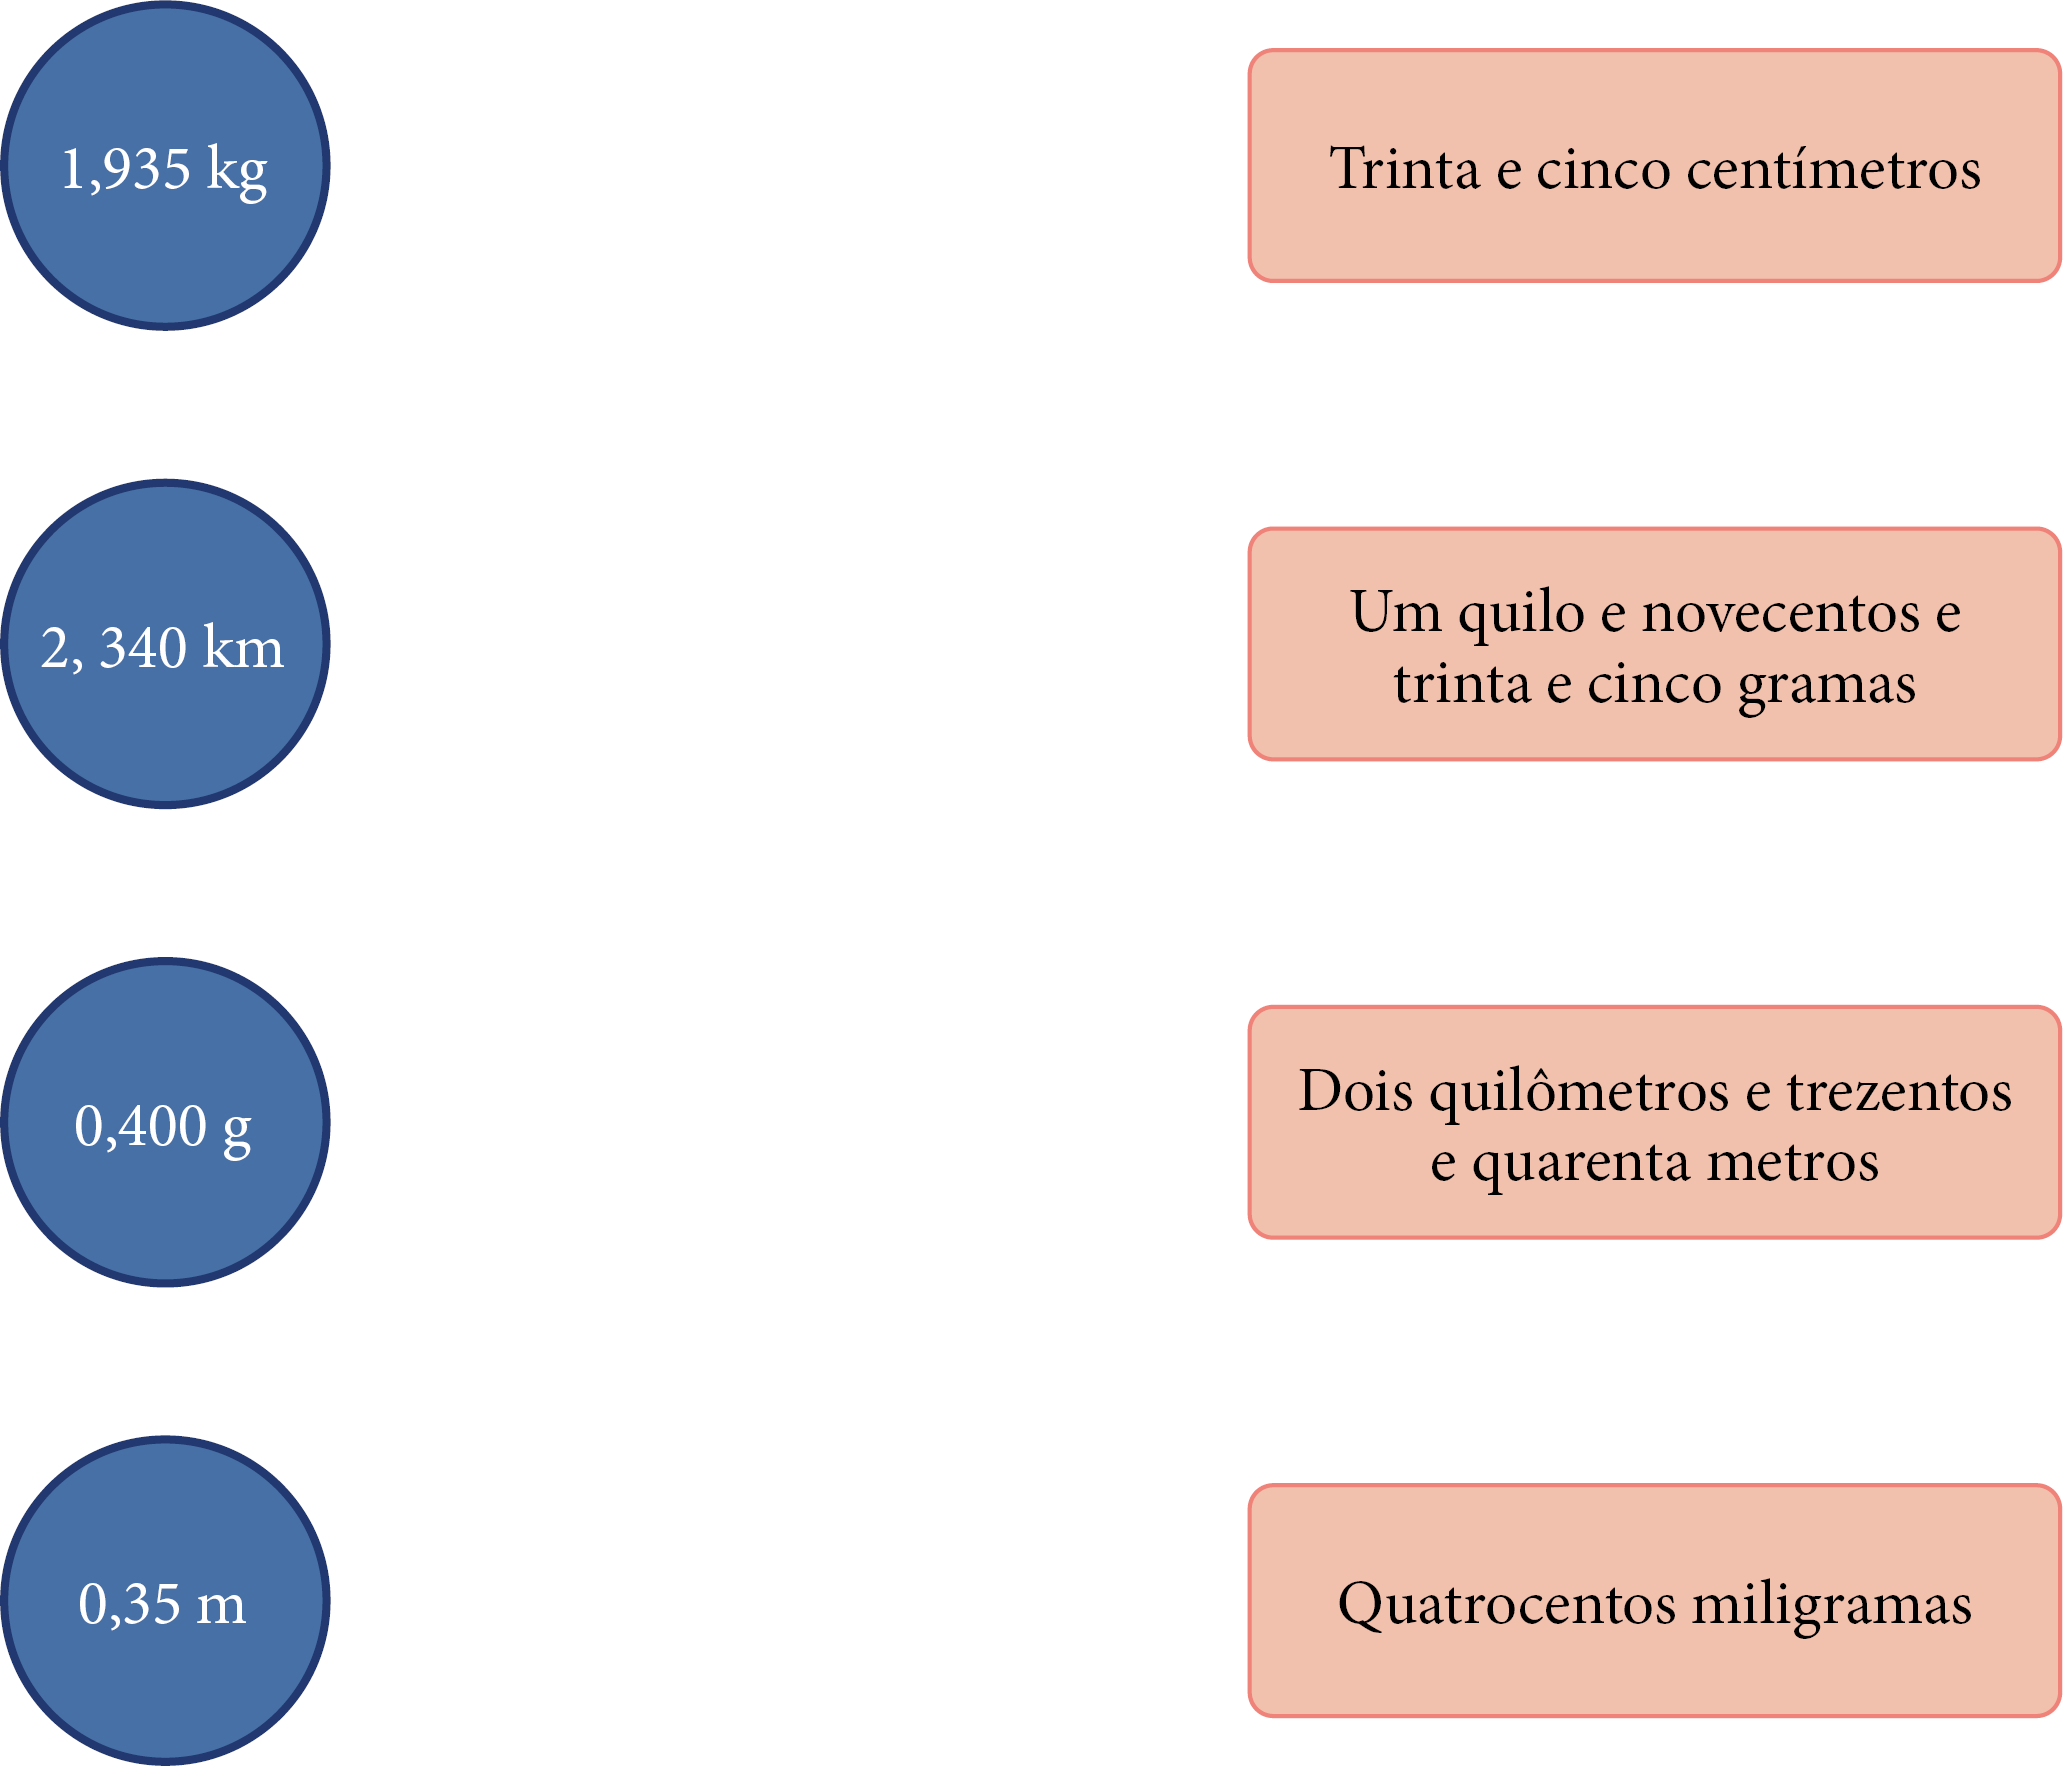
\includegraphics[width=\textwidth]{media/image20.png}
\end{figure}

%Respostas:
%1,935 kg = um quilo e novecentos e trinta e cinco gramas.
%2,340 km = Dois quilômetros e trezentos e quarenta metros.
%0,400 g = quatrocentos miligramas.
%0,35 m = trinta e cinco centímetros.

\num{2} Para cada item a seguir, forneça o número de décadas correspondente.

\begin{escolha}
\item Hipopótamo: vive em média 40 anos.

\reduline{4 décadas.\hfill}

\item Camelo: vive em média 50 anos.

\reduline{5 décadas.\hfill}

\item Leão: vive em média 20 anos.

\reduline{2 décadas.\hfill}

\item Elefante: vive em média 70 anos.

\reduline{7 décadas.\hfill}

\item Tartaruga: vive em média 100 anos.

\reduline{10 décadas.\hfill}

\item Arara: vive em média 60 anos.

\reduline{6 décadas.\hfill}
\end{escolha}


\num{3} Pinte a bolinha que corresponde à capacidade total de líquido que há em cada caso.

\begin{figure}[htpb!]
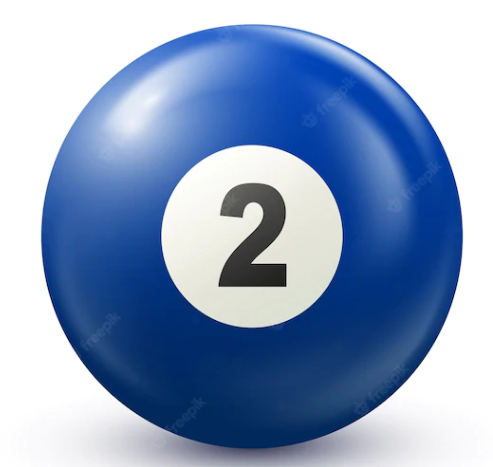
\includegraphics[width=.5\textwidth]{media/image21.png}
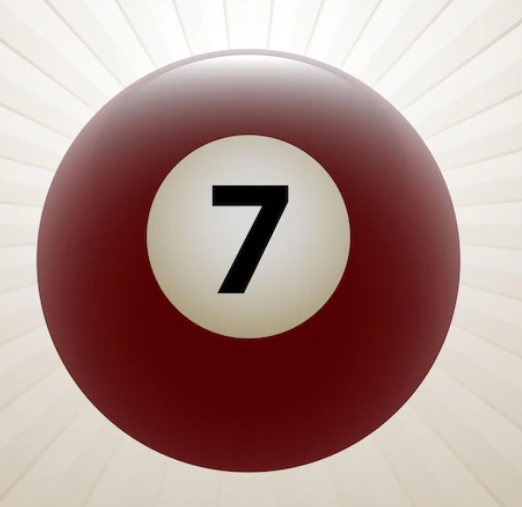
\includegraphics[width=.5\textwidth]{media/image22.png}
\end{figure}

\pagebreak
\begin{figure}[htpb!]

\includegraphics[width=.5\textwidth]{media/image23.png}
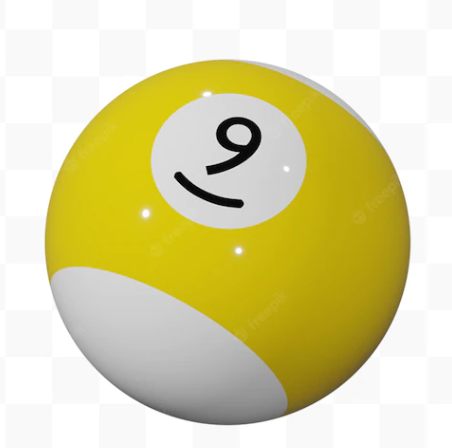
\includegraphics[width=.5\textwidth]{media/image24.png}
\end{figure}

%\coment{Duas unidades de limpador multiuso de 500 mL totalizam 1 litro. Três unidades de loção hidratante de 150 mL totalizam 450 mL (menos que 0,5 L). Quatro unidades de bebida energética de 330 mL totalizam 1.320 mL (menos que 1,5 L). Quatro unidades de amaciante de roupa de 1.000 mL totalizam 4.000 ml = 4 L (mais que 3,5 L).}

\num{4} A empresa em que Rafael trabalha vende suco de frutas com embalagens de
diversas capacidades: 200 mL, 250 mL, 333 mL e 1,5 L. Com base nisso, responda ao que se pergunta a seguir.

\begin{escolha}
\item Uma pessoa quer adquirir o volume de suco da maior embalagem,
  mas quer comprar a embalagem de 250 mL. Quantas embalagens deverão ser adquiridas?

\reduline{A embalagem maior possui 1.500 mL, o que corresponde a 6 embalagens de 250 mL.\hfill}

\item Oito embalagens de 250 mL equivalem a quantas embalagens de 200 mL?

\reduline{8 x 250 = 2.000 mL, o que equivale a 10 embalagens de 200 mL.\hfill}
\end{escolha}


\num{5} Um dos brinquedos do parque de diversões permanente de uma cidade proíbe
que crianças com uma altura menor que 1,20 m possam brincar em determinada
atração. Manoel mediu sua altura e ele está com 93 cm. Quanto ele
precisa crescer para poder realizar seu sonho de brincar nessa atração?

\begin{mdframed}[linewidth=2pt,linecolor=salmao,roundcorner=2pt]
\coment{1,20 m = 120 cm}\\
\coment{120 -- 93 = 23 cm}\\
\coment{Ele ainda precisará crescer 23 cm para que esteja apto a brincar na atração.}
\end{mdframed}

\num{6} Roberta utiliza um termômetro profissional para medir a temperatura da
água que vai utilizar para fazer uma deliciosa receita de rosca
caseira. A receita diz que a temperatura da água deve ser exatamente 74ºC
para que possa ser adicionada. Em determinado momento, Roberta colocou
o termômetro na água e observou a seguinte temperatura: 63ºC. Podemos concluir que

\begin{escolha}
\item
  Roberta já pode adicionar a água à receita.
\item
  A água está mais quente do que o necessário; sendo assim, será
  necessário esfriar um pouco para que possa ser adicionada.
\item
  A água está 11ºC abaixo da temperatura ideal; sendo assim, ainda
  precisa aquecer um pouco.
\item
  Roberta não tem dados para analisar se adiciona ou não a água à receita.
\end{escolha}

\coment{Como a temperatura indicada no termômetro é de 63ºC e a temperatura
ideal para a receita é de 74ºC, a água ainda deverá ser aquecida em 11ºC.}

\num{7} Observe as situações descritas a seguir e escreva o valor da massa (em quilogramas e em gramas) de cada item.

\begin{escolha}
\item
  Para equilibrar os pratos de uma balança para pesar um saco de tomates, foram colocados um peso de 1 kg, outro de 500 g e outro de 100 g.

  \reduline{1,6 kg = 1.600 g.\hfill}

\item
  Para equilibrar os pratos de uma balança para pesar um saco de batatas, foram colcoados um peso de 1 kg e outro de 500 g.

  \reduline{1,5 kg = 1.500 g.\hfill}

\item
  Para equilibrar os pratos de uma balança para pesar um saco de cenouras, foram colocados dois pesoas de 1 kg, um de 500 g, outro de 100 g e outro de 50 g.

  \reduline{2,65 kg = 2.650 g.\hfill}

\item
  Para equilibrar os pratos de uma balança para pesar um saco de cebolas, foram colocados um peso de 1 kg, dois pesos de 500 g, outro de 50 g e três outros de 10 g.

  \reduline{2,06 kg = 2.060 g.\hfill}
\end{escolha}

\num{8} Para a festa de aniversário de Arthur, seu pai encomendou 24 garrafas de
refrigerante. Dessas garrafas, 10 continham 3 litros (cada uma). Nas
demais garrafas, havia dois litros em cada uma. Com base nessas
informações responda ao que se pergunta a seguir.

\begin{escolha}
\item
  Qual é a quantidade de refrigerante, em mililitros, encomendada pelo pai de Arthur?

\reduline{(10 x 3) + (14 x 2) = 30 + 28 = 58 L = 58 000 mL.\hfill}

\item
  Se cada convidado da festa consumiu exatamente 400 mililitros de refrigerante e
  todo o refrigerante foi consumido durante a festa, quantas pessoas
  foram ao aniversário de Arthur?

\reduline{58.000 : 400 = 145 pessoas compareceram à festa.\hfill}
\end{escolha}

\num{9} O comprimento de uma escrivaninha é de 1,6 m. Quantos palmos,
aproximadamente, mede a escrivaninha se, em média, um palmo tem 23 cm?

\begin{minipage}{.5\textwidth}
\begin{escolha}
\item
  5 palmos.
\item
  6 palmos.
\item
  7 palmos.
\item
  8 palmos.
\end{escolha}
\end{minipage}
\sidetext{1,6 m = 160 cm.
160 : 23 = 6,95 palmos (aproximadamente 7 palmos).}

\num{10} Ana Luísa deve tomar um remédio de 8 em 8 horas. Se ela tomou o primeiro
comprimido às 6 horas da manhã, qual será o horário em que ela deverá tomar
o terceiro comprimido?

\begin{mdframed}[linewidth=2pt,linecolor=salmao,roundcorner=2pt]
\coment{Primeiro comprimido: 6 horas da manhã.}

\coment{Segundo comprimido: 6 + 8 = 2 horas da tarde ou 14 horas.}

\coment{Terceiro comprimido: 14 + 8 = 22 horas ou 10 horas da noite.}
\end{mdframed}


\section{Treino}

\num{1} Reinaldo foi contratado por uma empresa que possui um horário bem rígido.
Veja a seguir.

\begin{longtable}[]{@{}lll@{}}
\toprule
& Entrada & Saída\tabularnewline
\midrule
\endhead
Manhã & 8:00 & ?\tabularnewline
Tarde & 14:00 & 17:30\tabularnewline
\bottomrule
\end{longtable}


No período da manhã, Reinaldo deve
cumprir 4 horas e 30 minutos de trabalho. Qual será o horário em que
Reinaldo sairá para almoçar?

\begin{escolha}
\item
  11:00.
\item
  11:30.
\item
  12:00.
\item
  12:30.
\end{escolha}

\pagebreak
\num{2} Na receita médica de Marcela, recomenda-se que ela tome um xarope 4 vezes ao
dia e que, em cada vez, ela tome a quantidade de 8 mL durante 15 dias. Um
frasco do remédio contém 100 mL. Qual é a quantidade de
frascos que a mãe de Marcela deverpa comprar para que todo o tratamento
seja concluído?

\begin{escolha}
\item
  2.
\item
  3.
\item
  4.
\item
  5.
\end{escolha}


\num{3} Vicente teve de fazer uma viagem para fechar um grande negócio. Se o voo
saiu do aeroporto às 10 horas e 42 minutos e chegou ao destino às 14
horas e 8 minutos, qual foi o tempo de duração do voo?

\begin{escolha}
\item
  11.760 segundos.
\item
  9.542 segundos.
\item
  5.364 segundos.
\item
  2.500 segundos.
\end{escolha}


\chapter{Unidades e medidas}
\markboth{Módulo 5}{}

\section{Habilidades do SAEB}

\begin{itemize}
\item Medir ou comparar perímetro ou área de figuras planas desenhadas em
malha quadriculada.
\item Identificar horas em relógios analógicos ou associar horas em relógios
analógicos e digitais.
\item Resolver problemas que envolvam perímetro de figuras planas.
\item Resolver problemas que envolvam área de figuras planas.
\end{itemize}

\subsection{Habilidades da BNCC}

\begin{itemize}
\item EF04MA21, EF04MA22.
\end{itemize}

\conteudo{
Ampliação é o processo que realizamos quando queremos aumentar algo,
como, por exemplo, figuras planas, sem que suas características
sejam alteradas.

A figura menor a seguir teve o tamanho de todos os seus lados dobrado. Observe que manteve as mesmas
características.

Fazer a figura a seguir sem marcar os ângulos e a primeira deve ter lado
3 cm e a segunda lado 6 cm.

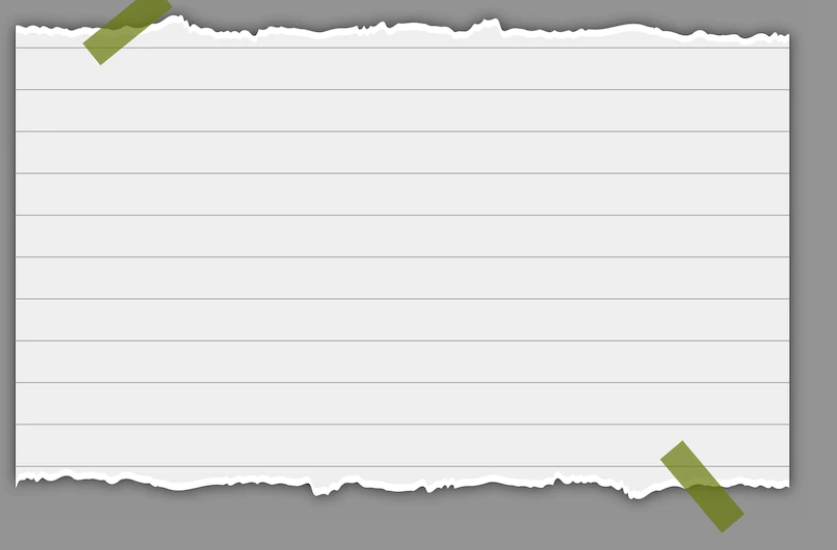
\includegraphics[width=.5\textwidth]{media/image25.png}

Redução é o processo que realizamos quando queremos diminuir algo,
como, por exemplo, figuras planas, sem que suas características
sejam alteradas.

A figura maior a seguir teve o tamanho de todos os seus lados dividido por dois. Observe que manteve as
mesmas características.

Fazer a figura a seguir sem marcar os ângulos e a primeira deve ter lado
6 cm e a segunda lado 3 cm.

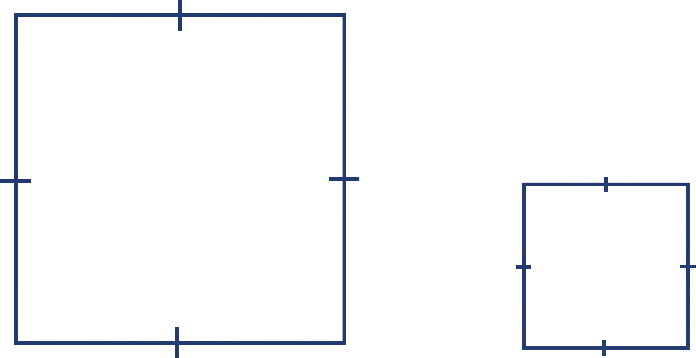
\includegraphics[width=.5\textwidth]{media/image26.png}

Muitas vezes, recorremos a malhas quadriculadas para nos
ajudar nesses processos. Com isso, é possível comparar áreas de
superfícies e até ter certeza de alguma ampliação ou alguma redução.

Outro instrumento muito útil é o relógio de ponteiros, que é dividido em doze partes ou
seções, numeradas de 1 a 12. Esses números representam as horas, marcadas pelo ponteiro menor.

Por sua vez, o intervalo de tempo que fica entre cada um dos números
representa a contagem dos minutos. Ficou convencionado que o
intervalo entre cada um deles é de 5 minutos. Então é necessário adicionar cinco minutos a cada número. Os minutos são marcados pelo ponteiro menor.
}

\section{Atividades}

\num{1} Aos finais de semana, Renato anda de bicicleta ao redor da praça
existente no bairro em que mora.
\pagebreak

\begin{figure}[htpb!]
\centering
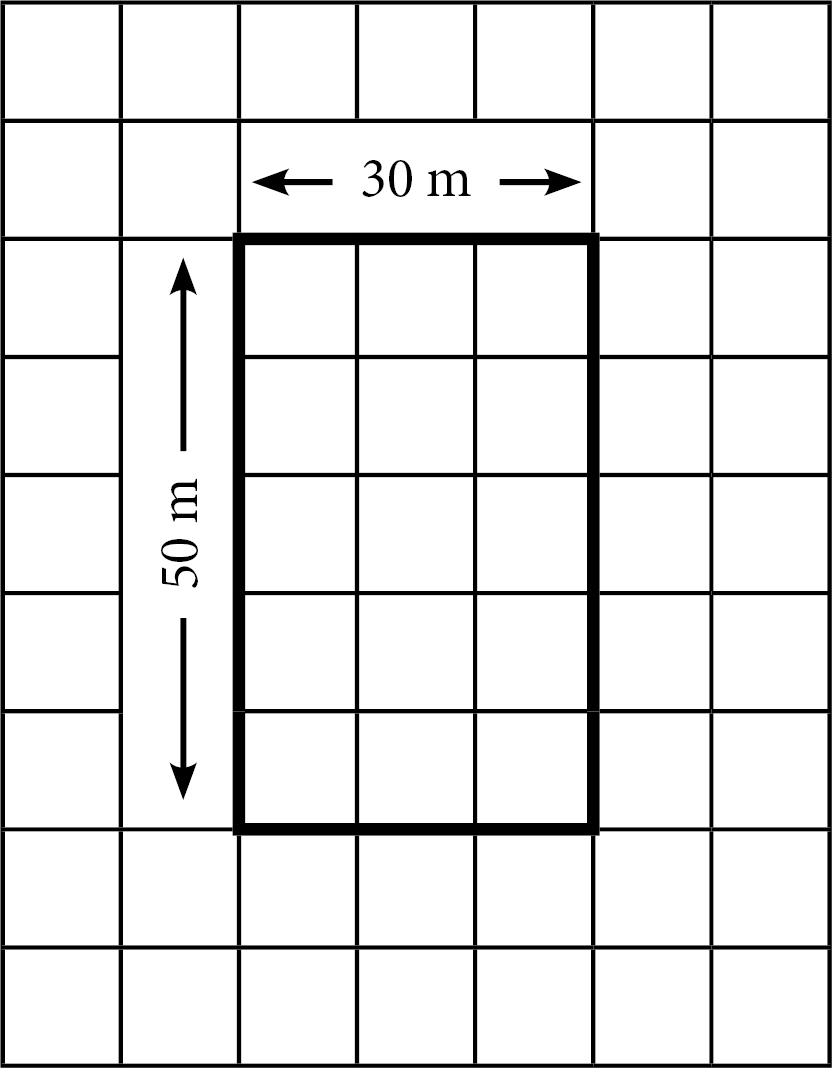
\includegraphics[width=.3\textwidth]{media/image27.png}
\end{figure}

Se ele der seis voltas completas ao redor da praça, ele percorrerá qual
distância em quilômetros?

\begin{mdframed}[linewidth=2pt,linecolor=salmao,roundcorner=2pt]
\coment{[(2 x 30) + (2 x 50)] x 6 = 960 m = 0,96 km.}\\
\coment{Sempre que possível, estimule a montagem da expressão para que os alunos comecem a se acostumar.}
\end{mdframed}


\num{2} Escreva por extenso as horas representadas a seguir. Depois, escreva uma atividade que você faz em cada um destes horários.

\begin{figure}[htpb!]
\centering
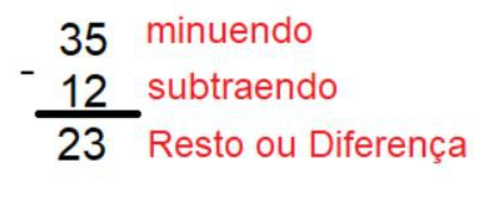
\includegraphics[width=.65\textwidth]{media/image28.png}
\end{figure}

\pagebreak
\num{3} Leandro resolveu cobrir de azulejos o fundo de sua piscina de tal forma
que apareça, no fundo, a letra inicial do nome de seu filho Arnaldo.
Sabendo-se que cada quadradinho corresponde a um azulejo de 3 metros
quadrados de área, qual é a área que os azulejos utilizados
ocuparão?

\begin{figure}[htpb!]
\centering
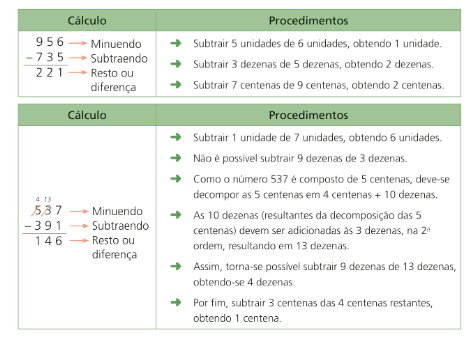
\includegraphics[width=.45\textwidth]{media/image29.png}
\end{figure}


\begin{mdframed}[linewidth=2pt,linecolor=salmao,roundcorner=2pt]
\coment{14 quadradinhos x 3 = 42 metros quadrados.}
\vspace*{1cm}
\end{mdframed}

\num{4} Escreva no espaço correspondente quantos meses compõem um período de:

\begin{escolha}
\item
  2 anos: \reduline{24 meses\hfill}

\item
  8 anos: \reduline{96 meses\hfill}

\item
  1 década: \reduline{120 meses\hfill}

\item
  1 século: \reduline{1.200 meses\hfill}
\end{escolha}

\num{5} Os desenhos representados a seguir representam as plantas baixas, inicial
e final, e o formato de uma praça que será construída em uma área
central de uma cidade. Inicialmente, a previsão era para uma praça
pequena, mas, como a prefeitura conseguiu uma área maior ao lado da
primeira, resolveu-se realizar a construção de uma praça maior.

\begin{figure}[htpb!]
\centering
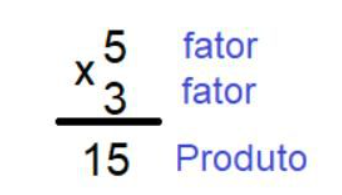
\includegraphics[width=\textwidth]{media/image30.png}
\end{figure}

Sendo assim, com relação à praça que se desejava construir iniciamente,
a nova praça terá uma área

\begin{multicols}{2}
\begin{escolha}
\item
  2 vezes maior.
\item
  3 vezes maior.
\item
  4 vezes maior.
\item
  5 vezes maior.
\end{escolha}
\end{multicols}

%A praça menor teria 6 quadradinhos preenchendo sua área, enquanto a grande terá 24 quadradinhos. Sendo assim, a área da praça maior é quatro vezes a área da praça menor.

\num{6} Observando-se atentamente as figuras, em que todos os quadradinhos têm a mesma área, pode-se perceber que a figura que possui a menor área é a

\begin{figure}[htpb!]
\centering
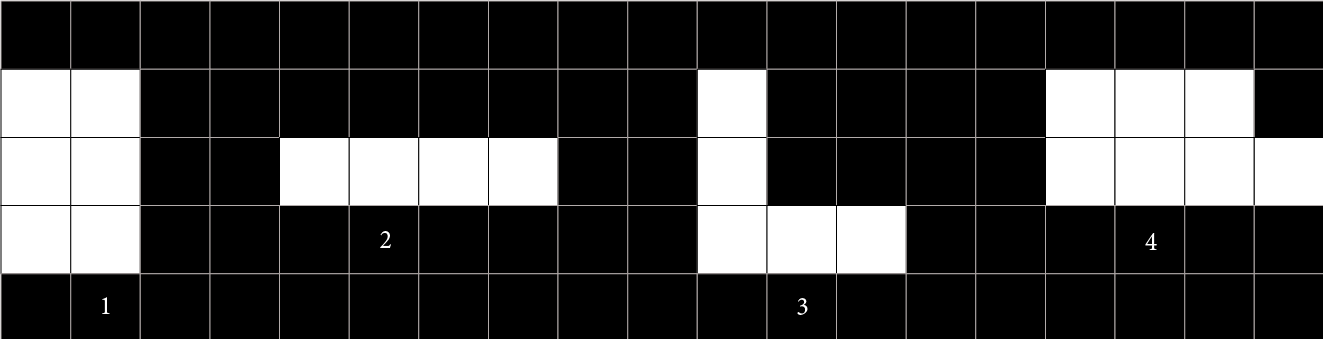
\includegraphics[width=\textwidth]{media/image31.png}
\end{figure}

\begin{multicols}{2}
\begin{escolha}
\item
  1.
\item
  2.
\item
  3.
\item
  4.
\end{escolha}
\end{multicols}
\pagebreak

%A figura 1 é composta de 6 quadradinhos. A figura 2 é composta de 4 quadradinhos. A figura 3 é composta de 5 quadradinhos. A figura 4 é composta de 7 quadradinhos. Como os quadradinhos são de mesmo tamanho, pode-se concluir que a figura que possui a menor área é a figura 2, por ser composta de um número menor de quadradinhos.

\num{7} Um arquiteto fez um primeiro esboço de uma construção no formato de cruz
que teria de executar.

\begin{figure}[htpb!]
\centering
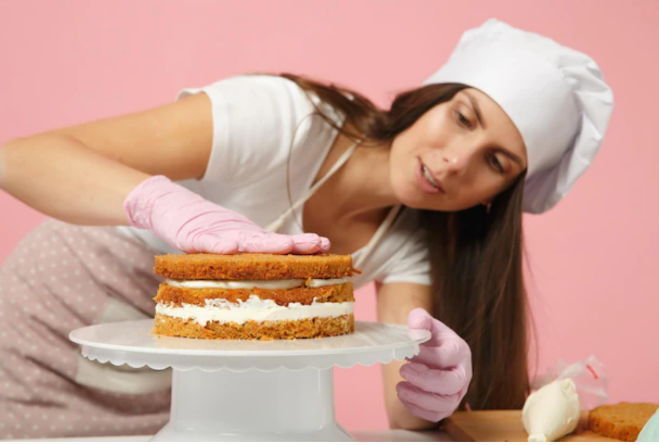
\includegraphics[width=\textwidth]{media/image32.png}
\end{figure}


No projeto final, todos os lados foram reduzidos à metade. Desenhe a nova imagem do projeto.

\begin{mdframed}[linewidth=2pt,linecolor=salmao,roundcorner=2pt]
\vspace{7cm}
\end{mdframed}

\num{8} Na malha quadriculada a seguir, cada quadrado representa uma área de 20
metros quadrados.

\begin{figure}[htpb!]
\centering
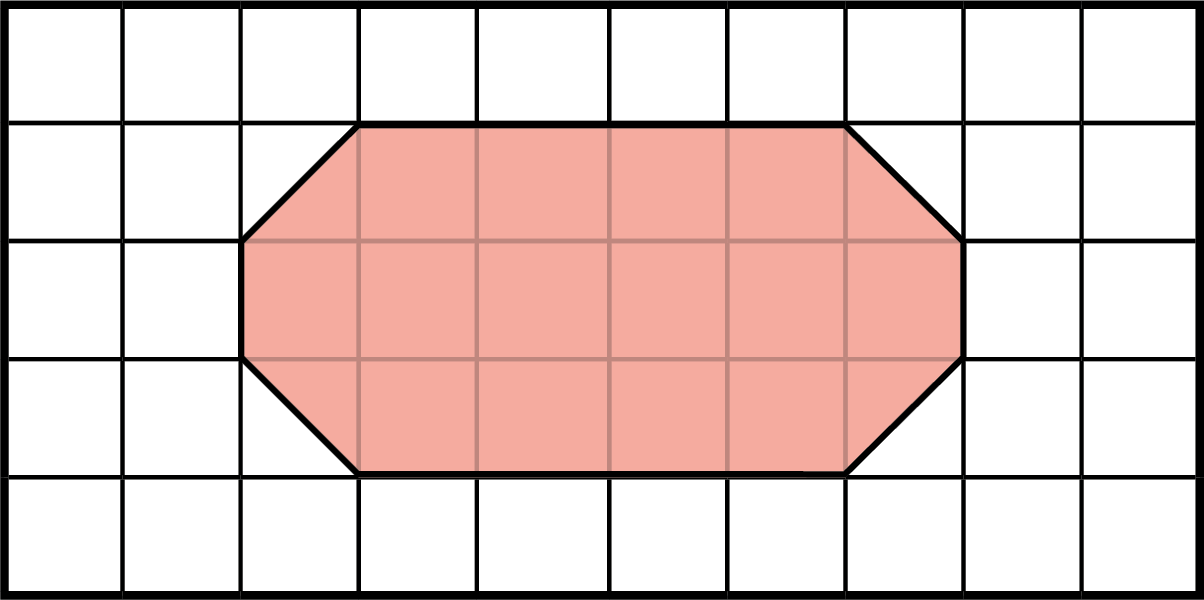
\includegraphics[width=\textwidth]{media/image33.png}
\end{figure}

Qual é a área da malha quadriculada que a figura destacada ocupa?

\begin{mdframed}[linewidth=2pt,linecolor=salmao,roundcorner=2pt]
\coment{Realizando-se a contagem de quadradinhos que preenchem a figura, chega-se
ao número 16. Portanto: 16 x 20 = 320 metros quadrados.}
\vspace{2cm}
\end{mdframed}

\num{9} Entre alguns objetos de seu irmão mais velho, Gabriel encontrou a seguinte
malha quadriculada com letras destacadas.

\begin{figure}[htpb!]
\centering
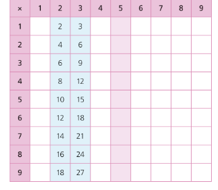
\includegraphics[width=.95\textwidth]{media/image34.png}
\end{figure}

\pagebreak

Entre essas letras, existem duas que ocupam superfícies de mesmo tamanho. Elas são a

\begin{escolha}
\item
  A e a C.
\item
  D e a E.
\item
  D e a C.
\item
  A e a E.
\end{escolha}

%Letra A: 14 quadradinhos.
%Letra C: 11 quadradinhos.
%Letra D: 13 quadradinhos.
%Letra E: 14 quadradinhos.
%As duas letras que ocupam asuperfícies de mesmo tamanho são a A e a E.

\num{10} Inês tem um compromisso inadiável às 20:25. Desenhe um relógio analógico
com os ponteiros indicando a hora do compromisso de Inês.

\begin{mdframed}[linewidth=2pt,linecolor=salmao,roundcorner=2pt]
\coment{O ponteiro menor deve estar um pouco depois do número 8, enquanto o ponteiro maior deve estar sobre o número 5.}
\vspace{11cm}
\end{mdframed}


\section{Treino}

\num{1} Paulo resolveu ir a uma exposição. Observe o mapa, em que cada quadradinho tem um lado que representa 2 metros na realidade.

\begin{figure}[htpb!]
\centering

\includegraphics[width=\textwidth]{media/image35.png}
\end{figure}

O caminho indicado é o de um corredor entre a bilheteria e o início da exposição.
Quanto ele precisará andar para chegar?

\begin{escolha}
\item
  8 m.
\item
  10 m.
\item
  12 m.
\item
  14 m.
\end{escolha}

\pagebreak
\num{2} Observe atentamente as figuras abaixo:

\begin{figure}[htpb!]
\centering
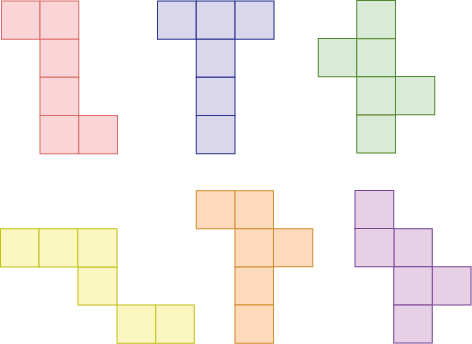
\includegraphics[width=.7\textwidth]{media/image36.png}
\end{figure}

Após a análise das figuras, percebe-se que:

\begin{escolha}
\item
  a primeira figura é a que possui a maior área.
\item
  a última figura é a que possui a menor área.
\item
  todas as figuras possuem a mesma área.
\item
  todas as figuras possuem áreas diferentes.
\end{escolha}

\num{3} Maria começou a se arrumar para um passeio com suas amigas na hora em
que, no relógio de seu quarto, o ponteiro menor estava entre o 11 e 12, enquanto o ponteiro maior estava sobre o 7. Ela terminou de se arrumar em 55 minutos. Que horário
o relógio estava marcando nesse segundo momento?

\begin{escolha}
\item
  11 horas e 50 minutos.
\item
  12 horas.
\item
  12 horas e 20 minutos.
\item
  12 horas e 30 minutos.
\end{escolha}


\chapter{O sistema monetário brasileiro}
\markboth{Módulo 6}{}

\section{Habilidades do SAEB}

\begin{itemize}
\item Relacionar valores de moedas e/ou cédulas do sistema monetário
brasileiro, com base nas imagens desses objetos.

\item Resolver problemas que envolvam moedas e/ou cédulas do sistema
monetário brasileiro.
\end{itemize}

\subsection{Habilidade da BNCC}

\begin{itemize}
  \item EF04MA25.
\end{itemize}

\conteudo{
Veja representações das cédulas e das moedas que usamos no Brasil.

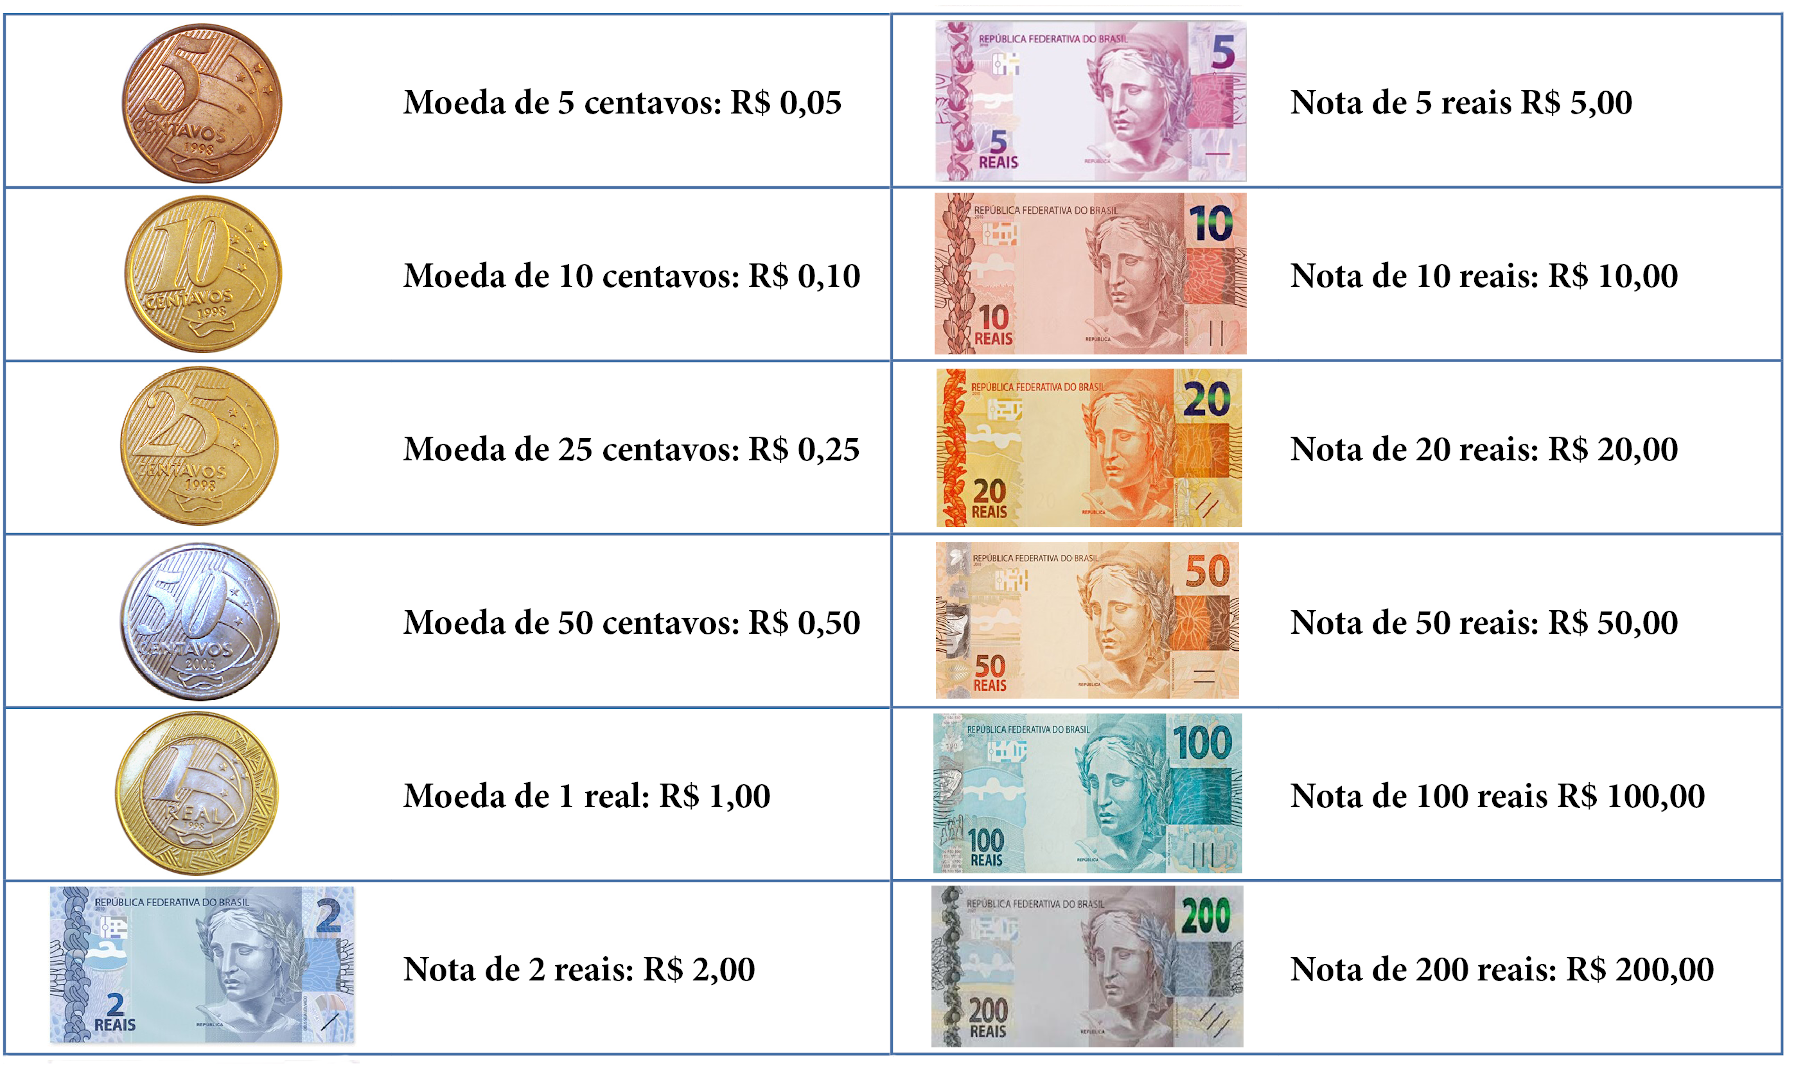
\includegraphics[width=\textwidth]{media/image37.png}
}

\section{Atividades}

\num{1} Marta foi à papelaria comprar uma caneta de que estava precisando para
continuar seus estudos. Ela comprou uma caneta que custava 7 reais e 25
centavos. Sabendo-se que ela pagou com uma nota de 10 reais, quais
cédulas e moedas ela recebeu de troco?

\reduline{Possibilidade de resposta: uma cédula de 2 reais, uma moeda de 50 centavos e uma moeda de 25 centavos.\hfill}
\linhas{2}

\num{2} Caíque economizou muito dinheiro, pois queria comprar um \textit{videogame} usado,
que custava R\$ 2.490,00 à vista. Ele conversou com o vendedor e pediu
um desconto extra e foi atendido com um desconto de R\$ 250,00. Quanto
ele pagou pelo \textit{videogame}?

\reduline{R\$ 2.490,00 -- R\$ 250,00 = R\$ 2.240,00.\hfill}
\linhas{2}

\num{3} Ainda com R\$ 4.000,00 na conta do banco, Ana tinha as seguintes contas para pagar em determinado dia do mês:

\begin{mdframed}[linewidth=2pt,linecolor=azul!20,backgroundcolor=azul!20,roundcorner=2pt]
\begin{itemize}
  \item Cartão de crédito: R\$ 1.128,00;
  \item Aluguel: R\$ 1.900,00;
  \item \textit{Petshop}: R\$ 480,00;
  \item Clube de assinatura: R\$ 635,00.
\end{itemize}
\end{mdframed}

Ana terá dinheiro suficiente para pagar todas as contas? Explique.

\reduline{Ana tem 1.128 + 1.900 + 480 + 635 = 4.143 reais de contas para pagar, mas só tem R\$ 4.000,00 na conta do banco, valor que é 143 reais menor do que o valor de ela precisa.\hfill}
\linhas{1}


\num{4} Em muitas compras a prazo, é exigida uma entrada que é paga no ato da
compra e o restante do valor pode ser dividido em um número combinado de
parcelas mensais. Veja o exemplo mostrado a seguir.

\begin{mdframed}[linewidth=2pt,linecolor=azul!20,backgroundcolor=azul!20,roundcorner=2pt]
Compre seu carro com uma entrada de R\$ 35.000,00 e 24
parcelas de R\$ 1.622,00.
\end{mdframed}

Agora, responda ao que se pergunta a seguir.

\begin{escolha}
\item
  Qual é o valor que será dividido em 24 vezes?

\reduline{24 x 1.622 = R\$ 38.928,00.\hfill}

\item
  Qual é o valor que cada parcela terá?

\reduline{R\$ 1.622,00.\hfill}

\item
  Se à vista a concessionária fornece um desconto de R\$ 4.580,00, quem optar por pagar à vista pagará quanto pelo carro?

\reduline{35.000 + (24 x 1.622) -- 4.580 = R\$ 69.348,00.\hfill}
\end{escolha}

\num{5} Responda ao que se pergunta a seguir, utilizando, em cada caso, o maior número possível de cédulas de cada valor.

\begin{escolha}
\item Com cédulas de 20, 10 e 2 reais, como se pode compor o valor R\$ 836,00?

\reduline{Quarenta e uma cédulas de 20 reais, uma cédula de 20 reais e três cédulas de 2 reais.\hfill}

\item Com cédulas de 200, 50 e 20 reais, como se pode compor o valor R\$ 3.940?

\reduline{Dezenove cédulas de 200 reais, duas cédulas de 50 reais e duas cédulas de 20 reais.\hfill}

\item Com cédulas de 100, 10 e 5 reais, como se pode compor o valor R\$ 1.735?

\reduline{Dezessete cédulas de 100 reais, três cédulas de 10 reais e uma cédula de 5 reais.\hfill}
\end{escolha}

\num{6} Em um restaurante, dois amigos pediram um prato feito, um prato executivo
e dois refrigerantes. O prato feito custa R\$ 22,00, o executivo custa R\$
28,00 e o refrigerante custa R\$ 6,00. Com três notas de vinte reais, eles
conseguem pagar a conta? Justifique a resposta com cálculos.

\begin{mdframed}[linewidth=2pt,linecolor=salmao,roundcorner=2pt]
\coment{22 + 28 + (2 x 6) = R\$ 62,00.}

\coment{Portanto 3 x 20 reais não serão suficientes para pagar a conta.}

\vspace{3cm}
\end{mdframed}

\num{7} Observe alguns preços de uma loja.

\begin{mdframed}[linewidth=2pt,linecolor=azul!20,backgroundcolor=azul!20,roundcorner=2pt]
\begin{itemize}
  \item \textbf{\textit{Notebook}}: R\$ 3.598,00.
  \item \textbf{\textit{Tablet}}: R\$ 1.680,00.
  \item \textbf{\textit{Smartphone}}: R\$ 2.640,00.
\end{itemize}
\end{mdframed}

Agora, responda ao que se pergunta a seguir.

\begin{escolha}
\item
  Quanto uma pessoa gastará se comprar um item de cada?

\reduline{3.598 + 1.680 + 2.640 = R\$ 7.918,00.\hfill}

\item
  Quantos reais o \textit{notebook} é mais caro que o \textit{tablet}?

\reduline{3.598 -- 1.680 = R\$ 1.918,00.\hfill}
\end{escolha}


\num{8} Mariana está pesquisando o preço de alguns itens de que está precisando e chegou aos resultados a seguir.

\begin{mdframed}[linewidth=2pt,linecolor=azul!20,backgroundcolor=azul!20,roundcorner=2pt]
\begin{itemize}
  \item Cola de bastão: R\$ 0,80.
  \item Rolo de fita adesiva: R\$ 0,50.
  \item Caneta ultrafina: R\$ 0,95.
  \item Borracha branca: R\$ 0,35.
\end{itemize}
\end{mdframed}

Agora, responda ao que se pergunta a seguir.

\begin{escolha}
\item
  Qual é a menor quantidade de moedas de 1 real de que ela necessitará para
  pagar por duas unidades de cada item?

\reduline{Preço a pagar: 2 x (0,80 + 0,50 + 0,95 + 0,35) = R\$ 5,20. Para esse valor, ela precisará de 6 moedas de 1 real.\hfill}

\item
  Qual é o troco que ele deverá receber nessa situação?

\reduline{Terá R\$ 0,80 de troco.\hfill}
\end{escolha}

\num{9} Uma rede de supermercados anunciou uma promoção com os produtos a seguir.

\begin{mdframed}[linewidth=2pt,linecolor=azul!20,backgroundcolor=azul!20,roundcorner=2pt]
\begin{itemize}
  \item Limpador multiuso: R\$ 3,75.
  \item Amaciante de roupa: R\$ 7,30.
  \item Água sanitária: R\$ 3,25.
  \item Desinfetante: R\$ 3,99.
  \item Desengordurante: R\$ 15,80.
\end{itemize}
\end{mdframed}

\pagebreak
Agora, faça o que se pede a seguir.

\begin{escolha}
\item
  Escreva como deve ser lido o preço de cada um dos produtos anunciados.

\reduline{R\$ 3,75: três reais e setenta e cinco centavos.\hfill}

\reduline{R\$ 7,30: sete reais e trinta centavos.\hfill}

\reduline{R\$ 3,25: três reais e vinte e cinco centavos.\hfill}

\reduline{R\$ 3,99: três reais e noventa e nove centavos.\hfill}

\reduline{R\$ 15,80: quinze reais e oitenta centavos.\hfill}

\item
  Construa uma sequência decrescente com os preços dos produtos anunciados.

\reduline{(15,80; 7,30; 3,99; 3,75; 3,25).\hfill}

\item
  Determine quantas notas de 20 reais são necessárias para adquirir uma unidade de cada produto anunciado.

\reduline{3,75 + 7,30 + 3,25 + 3,99 + 15,80 = R\$ 34,09; portanto são necessárias duas notas de 20 reais.\hfill}

\item
  Determine qual será o troco na situação apresentada no item anterior.

\reduline{40 -- 34,09 = R\$ 5,91 de troco.\hfill}
\end{escolha}

\num{10} Valentina vendeu alguns itens que não utilizava mais e como pagamento
recebeu um cheque em que estava escrito: doze mil quatrocentos e
cinquenta e nove reais. Como sua conta estava sem dinheiro algum, ela
resolveu depositar o cheque. No dia seguinte, realizou uma compra no
cartão de débito no valor de RS 12.305,92. Após essa operação qual será o
saldo de Valentina em sua conta bancária?

\coment{R\$ 12.459,00 -- R\$ 12.305,92 = R\$ 153,08.}

\section{Treino}

\num{1} Maria Luísa resolveu trocar com seu primo Francisco as moedas que ganhou de seu avô por notas de
R\$ 2,00. Em seu cofre, havia doze moedas de R\$ 0,50
e oito moedas de R\$ 0,25. Quantas cédulas Maria Luísa recebeu de Francisco?

\begin{escolha}
\item
  4.
\item
  6.
\item
  8.
\item
  20.
\end{escolha}


\num{2} Letícia resolveu arrumar o que estava em sua bolsa e encontrou
os seguintes valores: uma cédula de R\$ 5,00, duas cédulas de R\$ 2,00, uma moeda de R\$ 0,50, uma moeda de R\$ 0,25, três moedas de R\$ 0,10 e duas moedas de R\$ 0,05. No total, Letícia possui

\begin{escolha}
\item
  R\$ 9,00.
\item
  R\$ 9,90.
\item
  R\$ 10,10.
\item
  R\$ 10,15.
\end{escolha}

\pagebreak

\num{3} Na lanchonete a que Augusto costuma ir com seus amigos, existe a tabela de preços a seguir.

\begin{longtable}[]{@{}ll@{}}
\toprule
Produto & Valor por unidade\tabularnewline
\midrule
\endhead
Pão de queijo & R\$ 3,00\tabularnewline
Bombom & R\$ 5,00\tabularnewline
Suco & R\$ 6,00\tabularnewline
Sobremesa do dia & R\$ 4,50\tabularnewline
Refrigerante & R\$ 4,50\tabularnewline
Cachorro-quente & R\$ 12,00\tabularnewline
\bottomrule
\end{longtable}

Na última vez em que Augusto foi a esse lugar, ele comprou 4 bombons, 2
sucos e 3 cachorros-quentes. Qual é o valor gasto por Augusto nesse dia?

\begin{escolha}
\item
  R\$ 20,00.
\item
  R\$ 23,00.
\item
  R\$ 68,00.
\item
  R\$ 73,00.
\end{escolha}


\chapter{Qual é a probabilidade?}
\markboth{Módulo 7}{}

\section{Habilidades do SAEB}

\begin{itemize}
\item Identificar, entre eventos aleatórios, aqueles que têm menos, maiores ou
iguais chances de ocorrência, sem utilizar frações.

\item Determinar a probabilidade de ocorrência de um resultado em eventos
aleatórios, quando todos os resultados possíveis têm a mesma chance de
ocorrer (equiprováveis).
\end{itemize}

\subsection{Habilidade da BNCC}

\begin{itemize}
\item EF04MA26.
\end{itemize}

\conteudo{
Probabilidade é a chance de determinado
resultado ocorrer. O número 0 representa ``nenhuma chance'', enquanto o número 1
corresponde a ``chance certa''.

Quando se fala e probabilidade, é importante pensar nos fenômenos aleatórios, ou seja, aqueles cujo resultado não pode ser determinado mesmo se conhecendo todos os resultados possíveis. Por falar nisso, espaço amostral é o conjunto desses resultados.
}

\pagebreak
\section{Atividades}

\num{1} Em um estojo, há 25 lápis coloridos e 18 lápis pretos. Retirando-se, ao
acaso, um lápis desse estojo, o que tem chance maior: retirar um lápis
colorido ou um preto? Justifique sua resposta.

\begin{mdframed}[linewidth=2pt,linecolor=salmao,roundcorner=2pt]
\coment{Como há mais lápis coloridos do que pretos no estojo, a maior chance,
quando se retira um único lápis desse estojo, é que saia um lápis
colorido.}
\vspace{2cm}
\end{mdframed}

\num{2} Daniel joga um dado honesto. Sobre isso, determine as chances mencionadas a seguir.

\begin{escolha}
\item
  Tirar, na face voltada para cima, um número par.

\reduline{Temos sempre 6 possibilidades de números que podem sair: 1, 2, 3, 4, 5 e 6. Se interessa um número par, há três chances de isso acontecer (2, 4, 6).\hfill}

\item
  Tirar, na face voltada para cima, um número ímpar.

\reduline{Temos sempre 6 possibilidades de números que podem sair: 1, 2, 3, 4, 5 e 6. Se interessa um número ímpar, há três chances de isso acontecer (1, 3, 5).\hfill}

\item
  Tirar, na face voltada para cima, um número menor que 3.

\reduline{Temos sempre 6 possibilidades de números que podem sair: 1, 2, 3, 4, 5 e 6. Se interessa um número menor que 3, há duas chances de isso acontecer (1, 2).\hfill}
\end{escolha}

\num{3} Uma sacola escura, que não permite visualizar o que há dentro, contém
50 bolas idênticas, mas de cores diferentes. Sabe-se que 16 são azuis,
18 são pretas, 14 são vermelhas e 2 são amarelas. Calcule as chances de
acontecer o que se prevê a seguir.

\begin{escolha}
\item
  Que cor tem mais chance de aparecer quando se retira uma bola ao acaso? Justifique sua resposta.

\reduline{A maior probabilidade é de sair uma bola preta, porque é a cor que mais aparece na sacola.\hfill}

\item
  Há mais chance de sair um bola azul ou uma bola vermelha da sacola? Justifique sua resposta.

\reduline{Há mais chance de sair uma bola azul, porque há mais bolas azuis que vermelhas.\hfill}

\item
  Retirando-se uma bola ao acaso, a probabilidade de sair amarela é maior do que a de sair qualquer
  outra cor?

\reduline{Não, pois a probabilidade de sair uma amarela é a menor entre as
  probabilidades de saírem as outras cores, visto que a quantidade de
  bolas amarelas é a menor de todas.\hfill}
\end{escolha}


\num{4} Lucas tem guardado em uma caixa 16 livros de Matemática, 6 de História e
8 de Geografia. Retirando ao acaso um desses livros da caixa, responda ao que se pergunta a seguir.

\begin{escolha}
\item
  Qual livro tem mais chance de sair?

\reduline{Um livro de Matemática.\hfill}

\item
  Qual livro tem menos chance de sair?

\reduline{Um livro de História.\hfill}

\item
  Qual é a chance de sair uma livro de Língua Portuguesa?

\reduline{Não há chance de sair um livro de Língua Portuguesa, porque não há livros desse tipo na caixa.\hfill}
\end{escolha}

\pagebreak
\num{5} Na sala em que Clarissa estuda há 26 alunos, dos quais 18 são meninas. A
professora vai escolher um aluno para verificar se esse aluno fez a tarefa.
Uma menina ou um menino é mais provável que vai ser escolhido? Justifique sua resposta.

\begin{mdframed}[linewidth=2pt,linecolor=salmao,roundcorner=2pt]
\coment{Total de alunos: 26}

\coment{Número de meninas: 18}

\coment{Número de meninos: 26 -- 18 = 8}

\coment{É mais provável que seja escolhida uma menina.}
\end{mdframed}

\num{6} Uma letra é escolhida ao acaso entre as que formam a palavra
FUNDAMENTAL. É mais provável que a letra escolhida seja uma vogal ou uma consoante?

\begin{mdframed}[linewidth=2pt,linecolor=salmao,roundcorner=2pt]
\coment{Total de letras: 11}

\coment{Consoantes: 7}

\coment{Vogais: 11 -- 7 = 4}

\coment{Há mais chance de sair uma consoante.}
\end{mdframed}

\num{7} O baralho convencional é composto de 52 cartas divididas igualmente em quatro
naipes (copas, paus, ouros e espadas). Retirada uma carta ao acaso de um baralho,
qual naipe é mais provável de sair? Justifique sua resposta.

\reduline{Como são 52 cartas divididas igualmente em quatro naipes, a chance de sair qualquer um dos naipes é sempre a mesma; portanto não há um naipe mais provável.\hfill}

\num{8} Vítor quer escolher um número para sua camiseta do time de futebol e ele
pode escolher qualquer número de 1 a 25. Quantas chances ele tem de
escolher um número maior que 8 e menor que 18?

\begin{mdframed}[linewidth=2pt,linecolor=salmao,roundcorner=2pt]
\coment{Total de números: 25}

\coment{Total de números que interessam: 9}

\coment{Há, portanto, nove chances de sair um número maior que 8 e menor que 18.}
\end{mdframed}

\num{9} Os 500 estudantes de um colégio responderam a uma pergunta sobre a
área de conhecimento preferida, entre Exatas, Humanas e
Biológicas. As respostas foram computadas e alguns dados foram colocados
na tabela a seguir.

\begin{center}
\begin{tabular}{c|ccc}
\hline
\multirow{2}{*}{Área} & \multicolumn{3}{c}{Sexo} \\ \cline{2-4} 
 & \multicolumn{1}{c|}{Masculino (M)} & \multicolumn{1}{c|}{Feminino (F)} & Total \\ \hline
Exatas (E) & \multicolumn{1}{c|}{120} & \multicolumn{1}{c|}{80} & 200 \\ \hline
Humanas (H) & \multicolumn{1}{c|}{45} & \multicolumn{1}{c|}{80} & 125 \\ \hline
Biológicas (B) & \multicolumn{1}{c|}{100} & \multicolumn{1}{c|}{75} & 175 \\ \hline
Total & \multicolumn{1}{c|}{265} & \multicolumn{1}{c|}{235} & 500 \\ \hline
\end{tabular}
\end{center}

Um estudante é escolhido ao acaso. Determine a probabilidade de esse
estudante preferir Humanas.

\begin{mdframed}[linewidth=2pt,linecolor=salmao,roundcorner=2pt]
\coment{Total de estudantes: 500}

\coment{Preferência por humanas: 125}

\coment{Há 125 chances em 500 de o estudante escolhido ao caso preferir Humanas.}
\end{mdframed}

\pagebreak
\num{10} Carlos possui duas urnas com bolas que só são diferenciadas pela cor. A
distribuição das bolas nas urnas por cor se encontra na tabela a
seguir.

\begin{longtable}[]{@{}lll@{}}
\toprule
Cor & Urna 1 & Urna 2\tabularnewline
\midrule
\endhead
Amarela & 4 & 0\tabularnewline
Azul & 3 & 1\tabularnewline
Branca & 2 & 2\tabularnewline
Verde & 1 & 3\tabularnewline
Vermelha & 0 & 4\tabularnewline
\bottomrule
\end{longtable}

Ele vai colocar todas as bolas dessas duas urnas em uma única urna 3. Em
seguida retirará uma bola, ao acaso, dessa terceira urna. Qual é o total de possibilidades e quantas chances ele tem de tirar uma bola verde?

\begin{mdframed}[linewidth=2pt,linecolor=salmao,roundcorner=2pt]
\coment{Total de bolas: 20 (possibilidades).}

\coment{Bolas verdes: 4 (chances).}

\vspace{1cm}
\end{mdframed}


\section{Treino}

\num{1} Mateus precisa ir ao dentista na próxima semana, sem ser um dia de final de semana. Escolhendo ao acaso um dia
qualquer da semana para ir ao dentista, qual é a probabilidade de Mateus
escolher uma quinta-feira?

\begin{escolha}
\item
  1 chance em sete.
\item
  2 chances em sete.
\item
  1 chance em cinco.
\item
  2 chances em cinco.
\end{escolha}


\num{2} Em determinado momento, um restaurante está com 28 clientes e 7
garçons. Sobre essa situação, pode-se afirmar corretamente que

\begin{escolha}
\item
  há mais garçons que clientes.
\item
  é mais provável escolher um garçom ao acaso.
\item
  é mais provável escolher um cliente ao acaso.
\item
  há chances iguais de ser escolhido ao acaso um cliente ou um garçom.
\end{escolha}


\num{3} Uma estação de rádio está promovendo um concurso que funciona da seguinte maneira: cada vez que um ouvinte acerta qual é a música mais tocada do dia, ganha um cupom para o sorteio final. Veja, a seguir, quantos cupons alguns ouvintes conseguiram ganhar.

\begin{mdframed}[linewidth=2pt,linecolor=azul!20,backgroundcolor=azul!20,roundcorner=2pt]
\begin{itemize}
  \item Rogéria: 12 cupons;
  \item Paulo: 21 cupons;
  \item Márcia: 29 cupons;
  \item Carlos: 18 cupons.
\end{itemize}
\end{mdframed}

Se todos esses cupons forem colocados em uma urna, da qual será sorteado uma única vez um único cupom, qual dessas pessoas tem mais chance de ser sorteada?

\begin{escolha}
\item
  Carlos.
\item
  Márcia.
\item
  Paulo.
\item
  Rogéria.
\end{escolha}


\chapter{Dados estatísticos}
\markboth{Módulo 8}{}

\section{Habilidades do SAEB}

\begin{itemize}
\item Ler/identificar ou comparar dados estatísticos expressos em tabelas
(simples ou de dupla entrada).

\item Ler/identificar ou comparar dados estatísticos expressos em gráficos
(barras simples ou agrupadas, colunas simples ou agrupadas, pictóricos
ou de linhas).

\item Resolver problemas que envolvam dados apresentados tabelas (simples ou
de dupla entrada) ou gráficos estatísticos (barras simples ou agrupadas,
colunas simples ou agrupadas, pictóricos ou de linhas).
\end{itemize}

\subsection{Habilidade da BNCC}

\begin{itemize}
\item EF04MA27.
\end{itemize}

\conteudo{
Veja, a seguir, alguns tipos de gráfico mais utilizados em estatística.

\begin{itemize}
\item
  Gráfico de colunas ou barras.
\end{itemize}

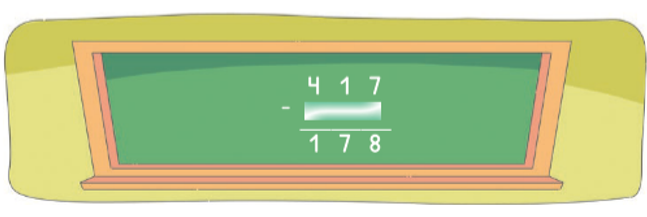
\includegraphics[width=.7\textwidth]{media/image38.png}

\begin{itemize}
\item
  Pictograma.
\end{itemize}

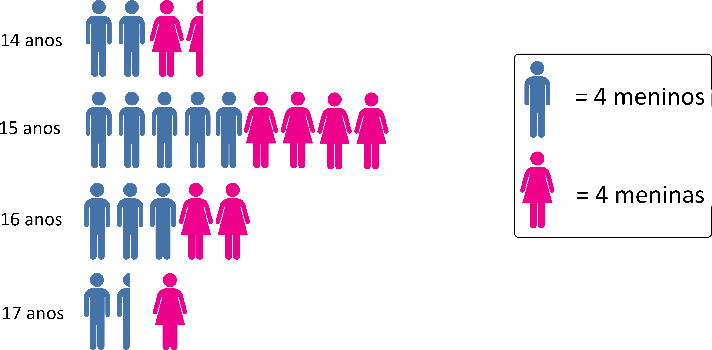
\includegraphics[width=\textwidth]{media/image39.png}

\begin{itemize}
\item
  Gráfico de linhas.
\end{itemize}

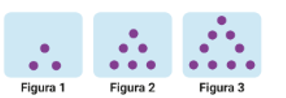
\includegraphics[width=\textwidth]{media/image40.png}

\pagebreak
\begin{itemize}
\item
  Gráfico de setores.
\end{itemize}

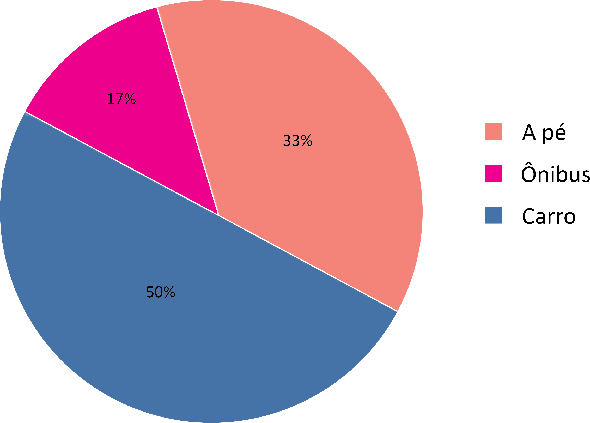
\includegraphics[width=\textwidth]{media/image41.png}
}

\section{Atividades}

\num{1} A tabela a seguir foi construída por uma escola com a finalidade de agrupar os
dados sobre a quantidades de alunos em alguns anos e o período em que
estudam. Observe.

\begin{longtable}[]{@{}lllll@{}}
\toprule
& 6º & 7º & 8º & 9º\tabularnewline
\midrule
\endhead
Período da manhã & 35 & 65 & 72 & 92\tabularnewline
Período da tarde & 54 & 43 & 48 & 43\tabularnewline
\bottomrule
\end{longtable}

\pagebreak
Quantos alunos o 6º ano do período da tarde tem a menos que o 9º
ano do período da manhã?

\begin{mdframed}[linewidth=2pt,linecolor=salmao,roundcorner=2pt]
\coment{92 -- 54 = 38. O 6º ano do períoda da tarde tem 38 alunos a
menos que o 9º do período da manhã.}
\vspace{2cm}
\end{mdframed}

\num{2} A OMS (Organização Mundial de Saúde) realizou uma pesquisa sobre o
consumo diário de água e os dados foram apresentados no gráfico a seguir.

\begin{figure}[htpb!]
\centering

\includegraphics[width=.9\textwidth]{media/image42.png}
\end{figure}

\pagebreak
Analisando-se atentamente o gráfico, qual é a diferença entre o
consumo diário de um europeu e de um brasileiro?

\begin{mdframed}[linewidth=2pt,linecolor=salmao,roundcorner=2pt]
\coment{200 -- 187 = 13 litros.}
\vspace{2cm}
\end{mdframed}

\num{3} Após todas as rodadas de um campeonato de futebol, os organizadores
apresentaram o gráfico a seguir sobre o número de pontos ganhos por cada
time.

\begin{figure}[htpb!]
\centering
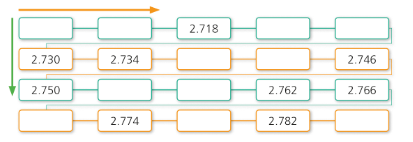
\includegraphics[width=.9\textwidth]{media/image43.png}
\end{figure}

Observando atentamente o gráfico, podemos concluir que o time B fez

\begin{escolha}
\item
  exatamente 50 pontos.
\item
  mais do que 40 pontos.
\item
  menos do que 25 pontos.
\item
  mais do que 30 pontos.
\end{escolha}

%O time B fez mais do que 30 pontos durante esse campeonato.

\num{4} Em uma empresa de doces, resolveu-se contratar um matemático que realizasse uma
pesquisa para verificar o tipo preferido de sobremesa das pessoas que
frequentavam determinado supermercado. Os entrevistados poderiam dar
apenas uma resposta entre as oferecidas na pesquisa. Após contagem dos
votos sobre a preferência, o matemático apresentou o gráfico a seguir
para a empresa que o contratou.

\begin{longtable}[]{@{}ll@{}}
\toprule
Sobremesa & Total de votos\tabularnewline
\midrule
\endhead
Pudim & 35\tabularnewline
Sorvete & 20\tabularnewline
Doce de leite & 22\tabularnewline
Goiabada com queijo & 10\tabularnewline
Salada de frutas & 13\tabularnewline
\bottomrule
\end{longtable}

Analisando o gráfico apresentado, responda ao que se pergunta a seguir.

\begin{escolha}
\item
  Qual foi a sobremesa menos votada?

\reduline{A sobremesa menos votada foi a goiabada com queijo.\hfill}

\item
  Qual foi a sobremesa mais votada?

\reduline{A sobremesa mais votada foi o pudim.\hfill}

\item
  Como fica uma sequência crescente dos números apresentados na tabela?

\reduline{(10; 13; 20; 22; 35).\hfill}

\item
  Após construir a sequência crescente, qual número ficou na posição
  central? A que sobremesa ele corresponde?

\reduline{O número que ocupa a posição central na sequência é o 20, que corresponde ao sorvete.\hfill}
\end{escolha}

\num{5} O professor de Educação Física apresentou os dados da quantidade de gols
marcados pelos 4 times que dispuraram o campeonato de futebol da escola no ano
corrente. Analise o gráfico e responda ao que se pergunta a seguir.

\begin{figure}[htpb!]
\centering

\includegraphics[width=.85\textwidth]{media/image44.png}
\end{figure}

\begin{escolha}
\item
  Qual turma fez a maior quantidade de gols? Qual foi a quantidade?

\reduline{A turma que fez a maior quantidade de gols foi a B, com 9 gols.\hfill}

\item
  Quais turmas fizeram um número de gols maior que 6?

\reduline{As turmas que fizeram um número de gols maior que 6 foram as turmas B e D.\hfill}

\item
  Qual turma fez a menor quantidade de gols?

\reduline{A turma C foi a que fez a menor quantidade de gols, pois marcou apenas 2 vezes.\hfill}
\end{escolha}

\pagebreak
\num{6} A tabela a seguir mostra parte do cadastro de uma escola.

\begin{figure}[htpb!]
\centering
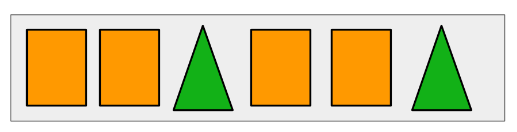
\includegraphics[width=\textwidth]{media/image45.png}
\end{figure}

Esse são os dados sobre o nascimento dos pais de quatro alunos da sala
de João. Analisando os dados, podemos perceber que a pessoa mais jovem,
entre as apresentadas na tabela, é

\begin{escolha}
\item
  Márcia.
\item
  Alex.
\item
  Samuel.
\item
  Aline.
\end{escolha}

%Como todos nasceram em abril do mesmo ano, a pessoa mais jovem será aquele que nasceu no maior valor que representa o dia. Sendo assim, o mais jovem é Samuel.

\pagebreak
\num{7} O governo realizou uma pesquisa sobre o número de queimadas que
ocorreram na Amazônia de 2007 a 2020. Analise o gráfico. Depois, faça o que se pede a seguir.


\begin{figure}[htpb!]
\centering
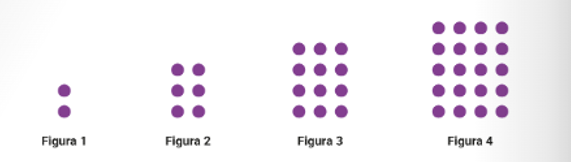
\includegraphics[width=\textwidth]{media/image46.png}
\end{figure}

\begin{escolha}
\item
  Pesquise o significado da sigla INPE, que aparece como fonte dos dados,
  e anote seu significado.

\reduline{INPE: Instituro Nacional de Pesquisas Espaciais.\hfill}

\item
  Escreva por extenso o ano em que mais ocorreram queimadas na Amazônia.

\reduline{Dois mil e sete foi o ano que apresentou a maior quantidade de queimadas na Amazônia.\hfill}

\item
  Determine os anos em que apareceu um número inferior a 1.500 queimadas na
  Amazônia.

\reduline{2008; 2009; 2011; 2013; 2015.\hfill}
\end{escolha}


\pagebreak
\num{8} Os dados fornecidos na tabela a seguir começaram ser passados para um
gráfico pictórico.

\begin{figure}[htpb!]
\centering
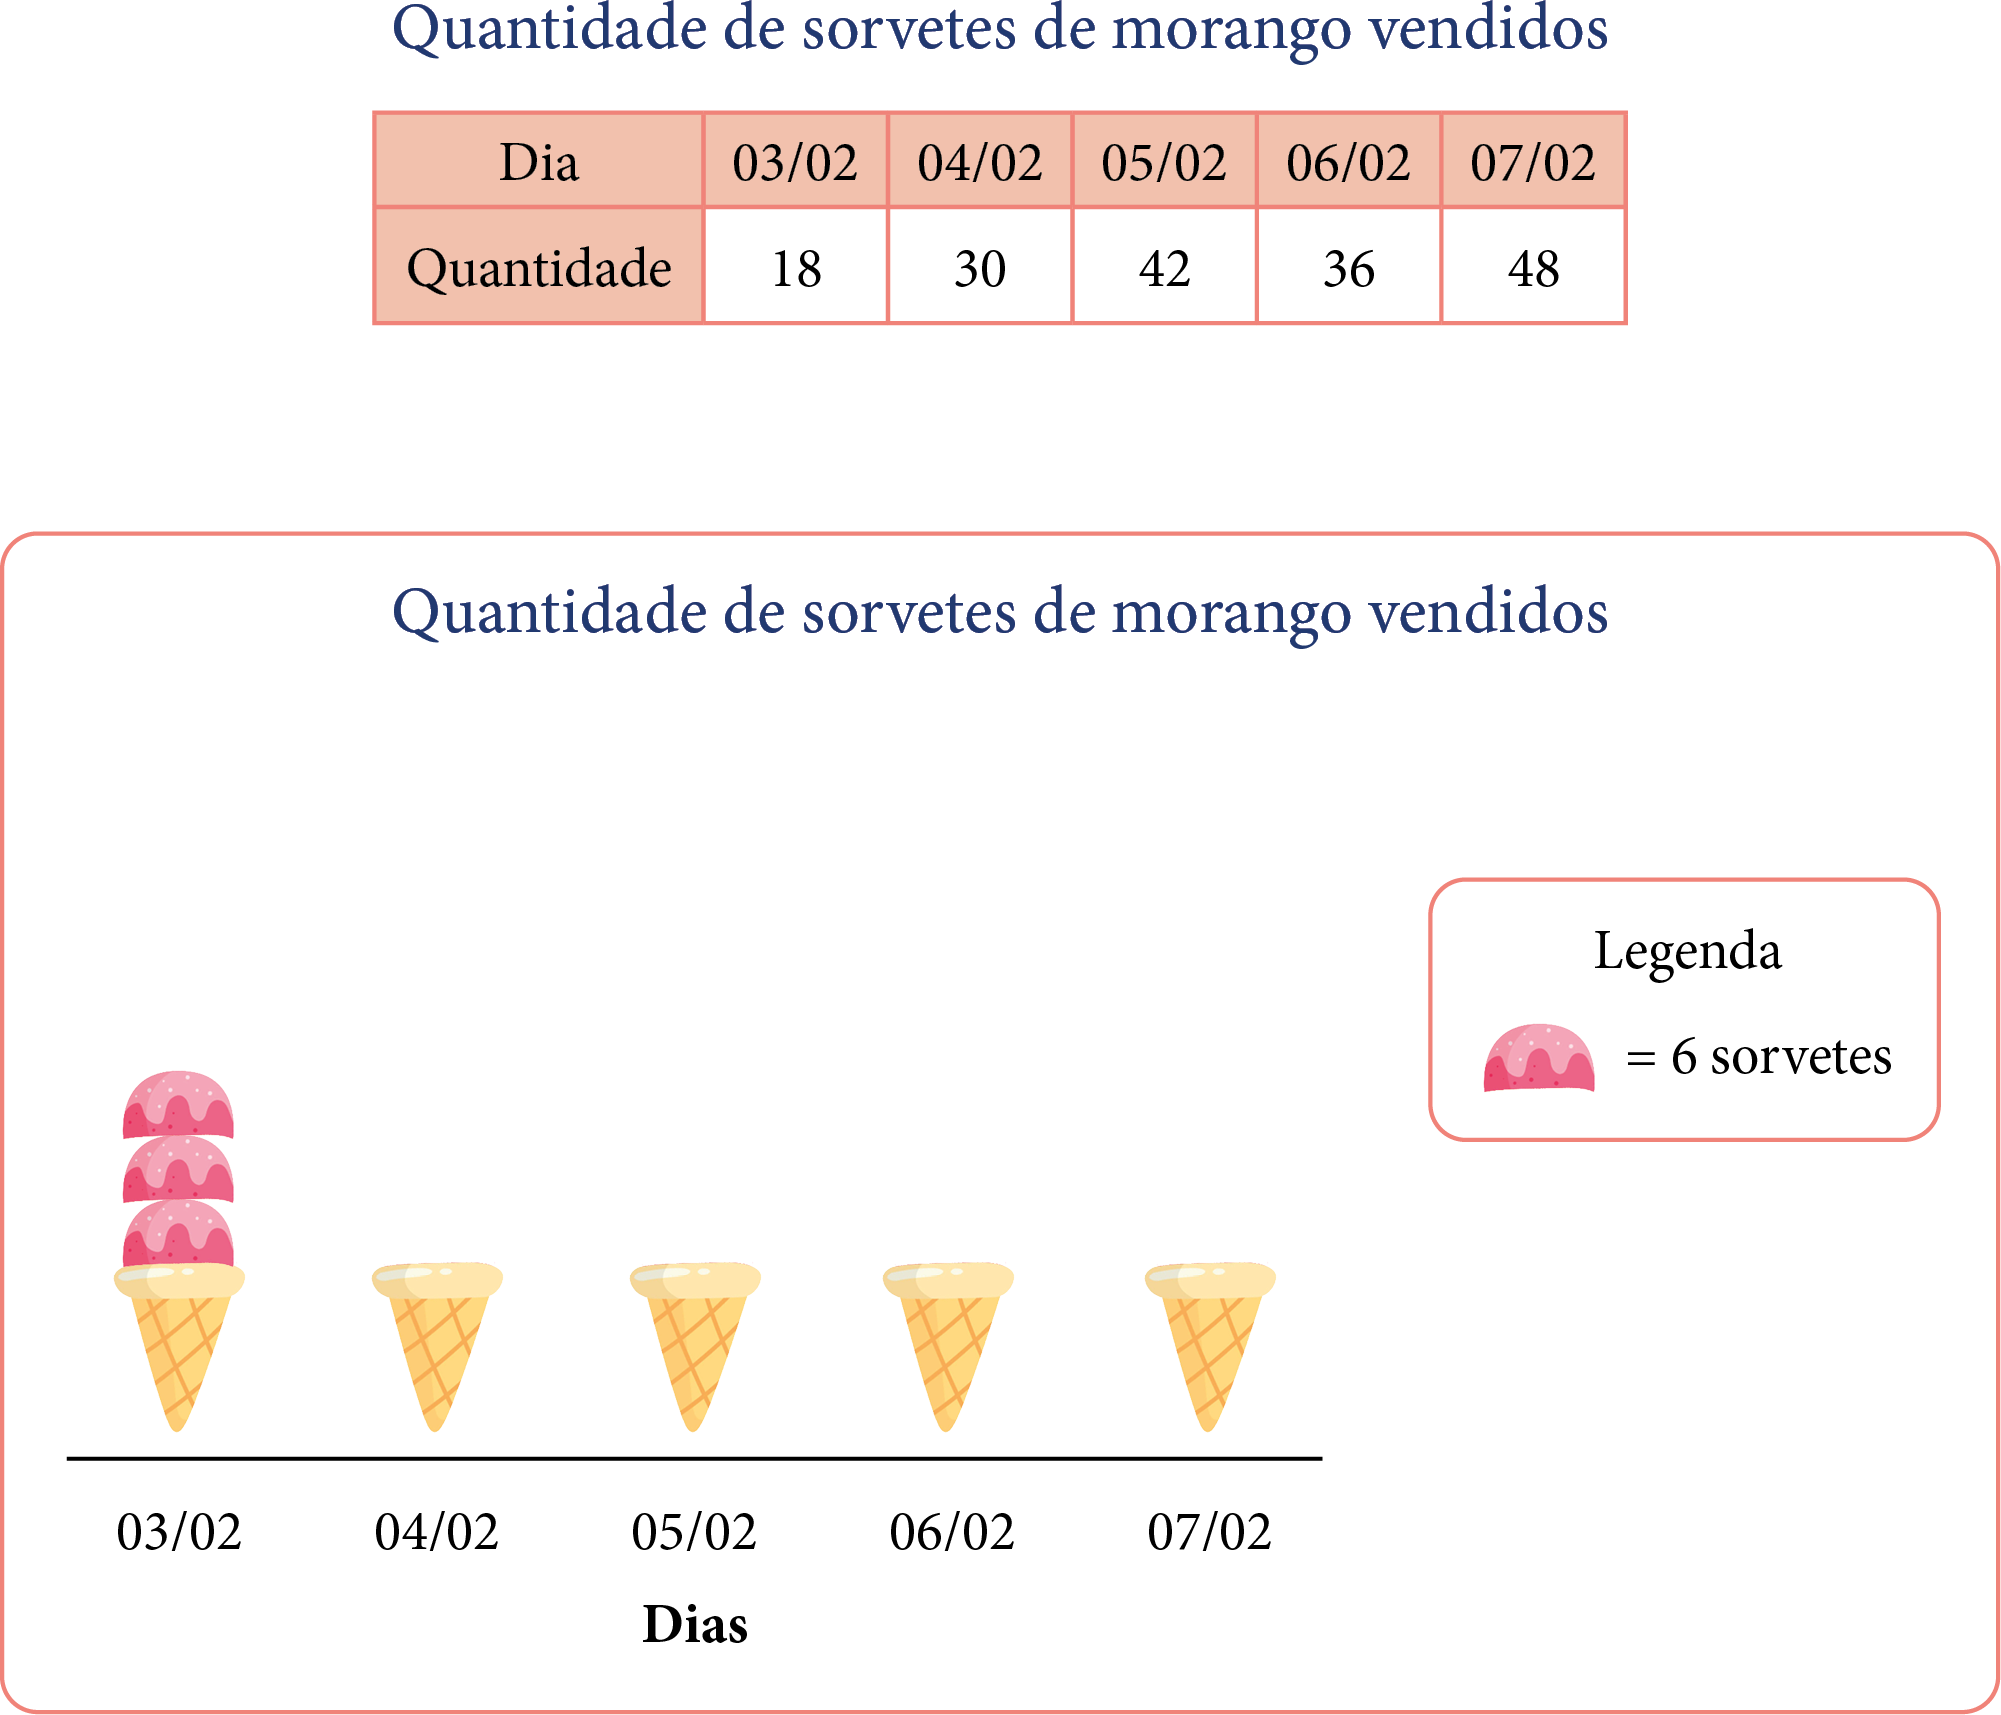
\includegraphics[width=\textwidth]{media/image47.png}
\end{figure}

Utilizando os dados da tabela e a legenda que o gráfico fornece,
complete o gráfico desenhando as bolas de sorvete que faltam.

%Resposta:
%$\frac{04}{02}$: 5 bolas de sorvete.
%$\frac{05}{02}$: 7 bolas de sorvete.
%$\frac{06}{02}$: 6 bolas de sorvete.
%$\frac{07}{02}$: 8 bolas de sorvete.

\pagebreak
\num{9} Utilizando conceitos modernos de educação, a professora de Leonardo
pediu que os alunos da turma realizassem uma pesquisa com 50 pessoas acerca da
preferência deles sobre determinados esportes. Sendo que cada pessoa
escolheu uma única opção, os dados da pesquisa foram colocados na tabela
a seguir.

\begin{figure}[htpb!]
\centering
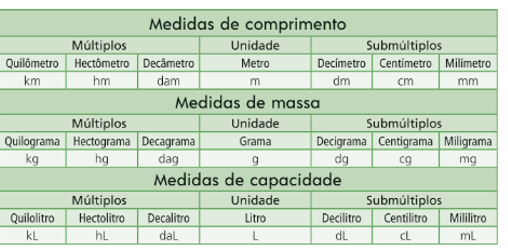
\includegraphics[width=\textwidth]{media/image48.png}
\end{figure}

Em seguida a professora pediu que os alunos contruíssem um gráfico de
colunas para representar os números da tabela. Construa o gráfico pedido
e ajude Leonardo a concluir a tarefa.

\begin{mdframed}[linewidth=2pt,linecolor=salmao,roundcorner=2pt]
\vspace{10cm}
\end{mdframed}

\num{10} Vanessa tem o hábito de realizar corridas diárias e construiu o seguinte
gráfico de barras com relação à distância percorrida em alguns dias. Observe atentamente o gráfico e responda ao que se pergunta a seguir.

\begin{figure}[htpb!]
\centering
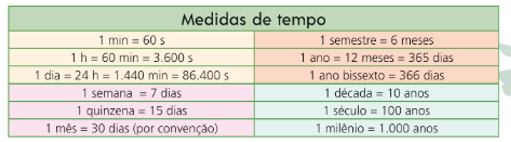
\includegraphics[width=\textwidth]{media/image49.png}
\end{figure}

\begin{escolha}
\item
  Em quais dias da semana ela percorreu a mesma distância?

\reduline{Na segunda-feira e na quinta-feira, ela percorreu a mesma distância: 14 km.\hfill}

\item
  Quantos quilômetros ela percorreu na sexta-feira?

\reduline{Na sexta-feira, ela percorreu 16 km.\hfill}

\item
  Em que dia ela percorreu exatamente 10 quilômetros?

\reduline{Na quarta-feira, ela percorreu 10 km.\hfill}

\item
  Quantos quilômetros, no total, ela percorreu nesses dias apresentados no gráfico?

\reduline{16 + (2 x 14) + 10 + 12 = 16 + 28 + 10 +12 = 66 km.\hfill}
\end{escolha}


\section{Treino}

\num{1} Pelas regras de um processo seletivo, o candidato que será aprovado será
aquele que tirar todas as notas acima de 30 e, além disso, obtiver o maior
número de notas iguais. As notas de 4 candidatos foram colocadas na
tabela a seguir.

\begin{longtable}[]{@{}lllll@{}}
\toprule
Candidato & Português & Matemática & Direito &
Informática\tabularnewline
\midrule
\endhead
A & 33 & 33 & 33 & 34\tabularnewline
B & 32 & 39 & 32 & 40\tabularnewline
C & 24 & 37 & 40 & 42\tabularnewline
D & 36 & 16 & 26 & 40\tabularnewline
\bottomrule
\end{longtable}

Segundo as regras do concurso, o que será aprovado é o candidato

\begin{multicols}{2}
\begin{escolha}
\item
  A.
\item
  B.
\item
  C.
\item
  D.
\end{escolha}
\end{multicols}



\num{2} Uma escola fez um levantamente sobre a quantidade de alunos em dois anos
do Ensino Fundamental. Os dados foram apresentados no gráfico a seguir.

\begin{figure}[htpb!]
\centering
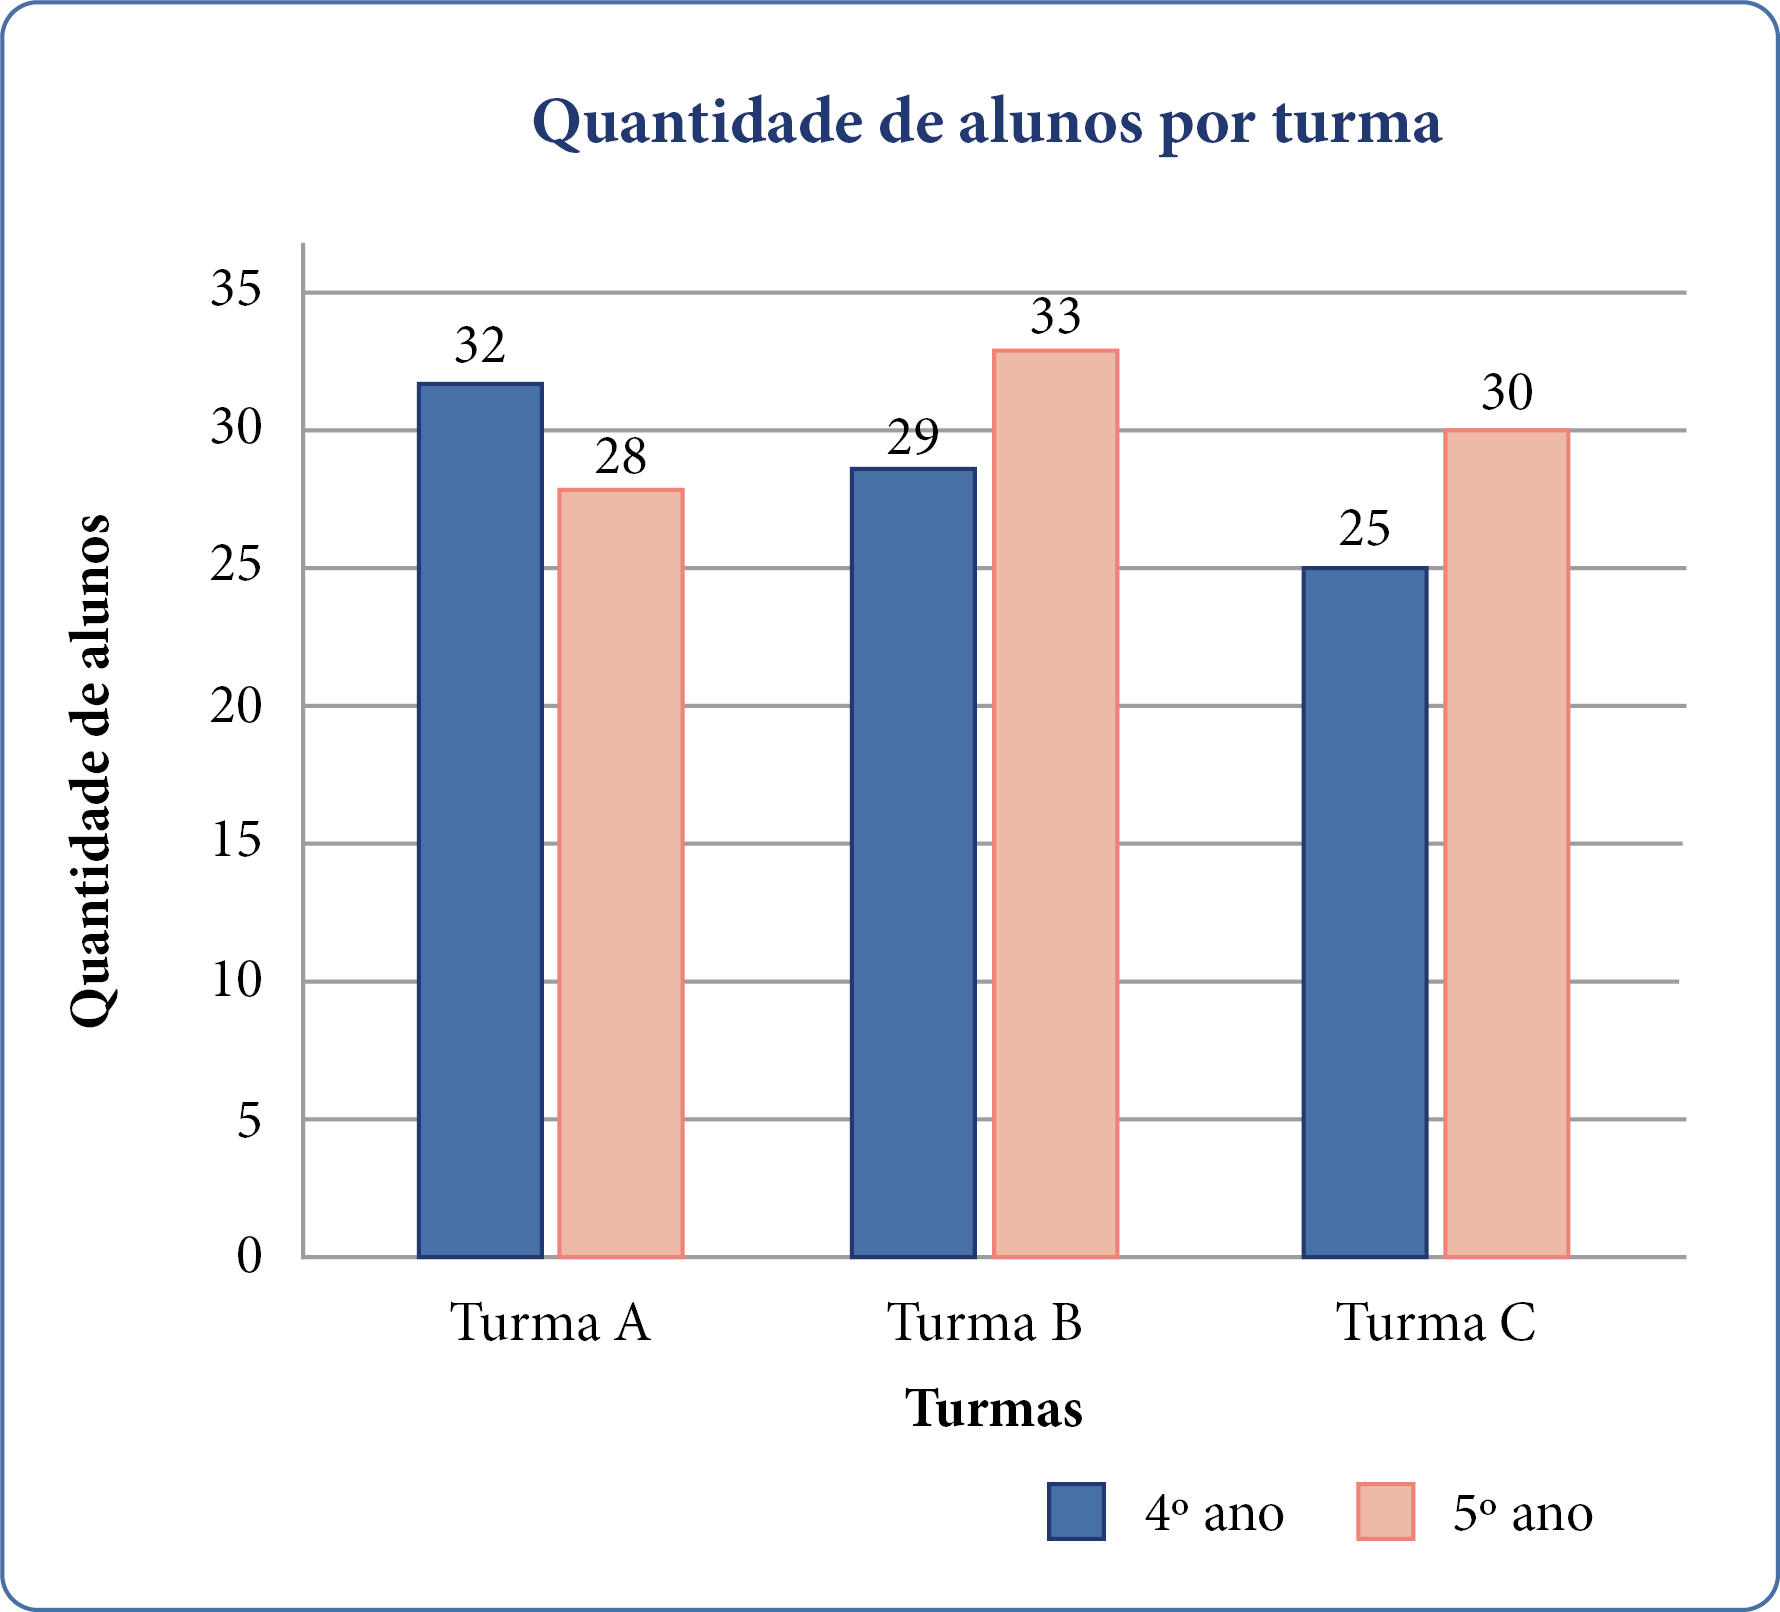
\includegraphics[width=.6\textwidth]{media/image50.png}
\end{figure}

Quantos alunos o 4º ano tem no total?

\begin{escolha}
\item
  60.
\item
  86.
\item
  91.
\item
  150.
\end{escolha}



\num{3} Uma loja de brinquedos efetuou uma pesquisa em determinado dia para
saber a faixa etária das crianças que visitaram a loja e os dados foram
colocados no gráfico a seguir.

\begin{figure}[htpb!]
\centering
\includegraphics[width=\textwidth]{media/image51.png}
\end{figure}

Pode-se afirmar que o total de crianças
de 7 a 12 anos que visitaram a loja é de

\begin{escolha}
\item
  7.
\item
  12.
\item
  16.
\item
  21.
\end{escolha}


\chapter{Partes do todo}
\markboth{Módulo 9}{}

\section{Habilidades do SAEB}

\begin{itemize}
\item Representar frações menores ou maiores que a unidade (por meio de
representações pictóricas) ou associar frações a representações pictóricas.

\item Identificar frações equivalentes.

\item Resolver problemas que envolvam fração como resultado de uma divisão
(quociente).

\item Resolver problemas que envolvam 10\%, 25\%, 50\%, 75\% e 100\%
associando essas representações, respectivamente, à décima parte, quarta parte, metade,
três quartos e um inteiro.
\end{itemize}

\subsection{Habilidade da BNCC}

\begin{itemize}
\item EF04MA09.
\end{itemize}

\conteudo{
As frações representam partes de um inteiro. Elas são formadas por dois números separados por uma barra. O número de cima é chamado de \textbf{numerador} e representa a quantidade de partes que temos, enquanto o número de baixo é chamado de \textbf{denominador} e representa a quantidade total de partes que o inteiro possui.

Por exemplo, se dividirmos uma pizza em oito partes iguais e pegarmos três dessas partes, podemos representar essa situação como a fração $\frac{3}{8}$. O numerador é 3, pois temos três partes da pizza, e o denominador é 8, pois a pizza foi dividida em oito partes iguais.

As frações podem ser comparadas entre si usando-se símbolos de ``igal a'', ``maior que'' ou ``menor que''. Por exemplo, $\frac{1}{2}$ é menor que $\frac{3}{4}$, pois metade de um inteiro é menor que três quartos do mesmo inteiro.

As frações também podem ser somadas ou subtraídas, desde que tenham o mesmo denominador. Para fazer isso, basta somar ou subtrair os numeradores e manter o denominador igual. Por exemplo, $\frac{1}{4}$ + $\frac{1}{4}$ = $\frac{2}{4}$.

As frações podem, ainda, ser simplificadas, ou seja, podemos dividir o numerador e o denominador por um mesmo número para obtermos uma fração equivalente. Por exemplo, $\frac{2}{4}$ pode ser simplificado dividindo-se o numerador e o denominador por 2, o que resulta em $\frac{1}{2}$.
}

\section{Atividades}

\num{1} Faça o que se pede em cada item.

\begin{escolha}
\item
Calcule a metade de 6.842: \reduline{3.421.\hfill}

\item
Calcule a terça parte de 43.863: \reduline{14.621.\hfill}

\item
Calcule a quinta parte de 12.195: \reduline{2.439.\hfill}

\item
Calcule a nona parte de 12.312: \reduline{1.368.\hfill}

\end{escolha}

\num{2} Uma escola, em período de Copa do Mundo, resolveu fornecer aos alunos um
álbum coletivo de figurinhas. Eles deveriam contribuir com o
preenchimento do álbum fornecendo as figurinhas. Sabe-se que Cássia
contribuiu com $\frac{1}{7}$ da quantidade total de figurinhas, enquanto Marcos
doou $\frac{2}{5}$ do total.

\begin{escolha}
\item
  Qual é a fração do total de figurinhas do álbum que os dois juntos doaram?

\reduline{$\frac{1}{7}$ + $\frac{2}{5}$ = $\frac{12}{35}$ do total de figurinhas foram doadas por Cássia e Marcos.\hfill}
\bigskip

\item
  Qual é a fração do total de figurinhas do álbum que ainda falta para que os alunos o completem?

\reduline{1 -- $\frac{12}{35}$ = $\frac{23}{35}$.\hfill}
\bigskip
\end{escolha}


\num{3} Durante uma campanha de recapeamento dos ruas de uma cidade, a rua em
que André mora começou a ser concertada. Até hoje $\frac{2}{9}$ dessa rua já foi mexido.
Qual é a fração da extensão total da rua que ainda falta para ser
recapeada? Já foi recapeado mais de $\frac{1}{3}$ da rua? Justifique sua resposta.

Deixar espaço em branco equivalente a 3 linhas para a resolução

\begin{mdframed}[linewidth=2pt,linecolor=salmao,roundcorner=2pt]
\coment{1 -- $\frac{2}{9}$ = $\frac{9}{9}$ -- $\frac{2}{9}$ = $\frac{7}{9}$ (parcela do que ainda precisa ser recepeado).}

\coment{Não foi recapeado mais de um terço, já que $\frac{1}{3}$ é equivalente a $\frac{3}{9}$, que é menor que $\frac{2}{9}$, parcela do que já foi recapeado.}
\vspace{2cm}
\end{mdframed}

\num{4} Em quais das figuras a seguir, a parte destacada representa $\frac{1}{2}$ do todo?

\begin{figure}[htpb!]
\centering
\includegraphics[width=\textwidth]{media/image52.png}
\end{figure}

\reduline{São as figuras 1, 3, 5 e 6\hfill}
\linhas{2}

\num{5} Em cada item a seguir, temos duas figuras. Analise com calma e escreva no espaço
entre elas se a primeira figura tem área pintada maior ou menor do que a
região destacada na segunda figura.

\begin{figure}[htpb!]
\centering
\includegraphics[width=\textwidth]{media/image53.png}
\end{figure}

\coment{Na primeira figura, temos $\frac{4}{9}$ pintado; na segunda, $\frac{3}{9}$. A área pintada da primeira é maior do que a área pintada da segunda. Na primeira figura, temos $\frac{5}{12}$ pintado; na segunda, $\frac{9}{12}$. A área pintada da primeira é menor do que a área pintada da segunda. Na primeira figura, temos $\frac{4}{15}$ pintado; na segunda, $\frac{7}{15}$. A área pintada da primeira é menor do que a área pintada da segunda.}

\pagebreak
\num{6} Pinte a quantidade de itens solicidada e escreva qual é a fração do total que você pintou.

\begin{escolha}
\item Um quarto das lapiseiras.

\includegraphics[width=\textwidth]{media/image54.png}

\coment{Como temos 32 lapiseiras e queremos pintar $\frac{1}{4}$ delas, deveremos pintar 8 lapiseiras.}

\item  Um terço das borrachas.

\includegraphics[width=\textwidth]{media/image55.png}

\coment{Como temos 48 borrachas e queremos pintas $\frac{1}{3}$ delas, deveremos pintar 16 borrachas.}

\item A quinta parte das canetas.

\includegraphics[width=\textwidth]{media/image56.png}

\coment{Como temos 35 canetas e queremos pintas $\frac{1}{5}$ delas, deveremos pintar 7 canetas.}

\item  Um décimo das bolas.

\includegraphics[width=.65\textwidth]{media/image57.png}

\coment{Como temos 30 bolas e queremos pintar $\frac{1}{10}$ delas, deveremos pintar 3 bolas.}
\end{escolha}

\num{7} Identifique a fração da figura estipulada em cada item, colorindo a
quantidade indicada. Em seguida, complete a frase com o número correto de
unidades que você pintou.

\begin{figure}[htpb!]
\includegraphics[width=\textwidth]{media/image58.png}
\end{figure}

\begin{figure}[htpb!]
\includegraphics[width=\textwidth]{media/image59.png}
\end{figure}

\begin{figure}[htpb!]
\includegraphics[width=\textwidth]{media/image60.png}
\end{figure}

\begin{figure}[htpb!]
\includegraphics[width=\textwidth]{media/image61.png}
\end{figure}

%\coment{Devem ser pintados 6 quadradinhos. Deve ser colocado o número 6 no espaço em branco.}
%\coment{Devem ser pintados 16 quadradinhos. Devem ser colocados os números 24 e 16, respectivamente, nos espaços em branco.}
%\coment{Devem ser pintados 8 retângulos. Devem ser colocados os números 16 e 8, respectivamente, nos espaços em branco.}
%\coment{Devem ser pintados 10 retângulos. Devem ser colocados os números 25 e 10, respectivamente, nos espaços em branco.}

\pagebreak
\num{8} Observe a quantidade total de ovos contida em cada uma das caixas
representadas nos itens a seguir e escreva, no local destinado, a fração que
representa os ovos de cada cor com relação ao total contido na caixa.

\begin{figure}[htpb!]
\centering
\includegraphics[width=.4\textwidth]{media/image62.png}
\includegraphics[width=.4\textwidth]{media/image63.png}
\end{figure}

\begin{figure}[htpb!]
\centering
\includegraphics[width=.4\textwidth]{media/image64.png}
\includegraphics[width=.4\textwidth]{media/image65.png}
\end{figure}

%\coment{Vermelhos: $\frac{12}{16}$ = $\frac{3}{4}$; azuis: $\frac{4}{16}$ = $\frac{1}{4}$.}
%\coment{Vermelhos: $\frac{12}{32}$ = $\frac{3}{8}$; azuis: $\frac{20}{32}$ = $\frac{5}{8}$.}
%\coment{Vermelhos: $\frac{10}{25}$ = $\frac{2}{5}$; azuis: $\frac{15}{25}$ = $\frac{3}{5}$.}
%\coment{Vermelhos: $\frac{15}{24}$ = $\frac{5}{8}$; azuis: $\frac{9}{24}$ = $\frac{3}{8}$.}

\num{9} Renato percebeu que, em sua coleção de cartas, havia $\frac{3}{5}$ do total delas
que eram de carros. Se a coleção dele tem, ao todo, 35 cartas, quantas são
as cartas de carros?

\begin{mdframed}[linewidth=2pt,linecolor=salmao,roundcorner=2pt]
\coment{$\frac{3}{5}$ de 35 = 3 x 7 = 21.}
\vspace{2cm}
\end{mdframed}

\num{10} Um centro comunitário resolveu realizar uma campanha do agasalho. Dos
100 agasalhos arrecadados, $\frac{12}{50}$ foram doados para uma instituição que
cuida de idosos. O restante foi doado a uma instituição que acolhe
crianças carentes. Agora, responda ao que se pergunta a seguir.

\begin{escolha}
\item
  Qual é a quantidade doada aos idosos?

\reduline{$\frac{12}{50}$ x 100 = 24 agasalhos para idosos.\hfill}

\item
  Qual é a quantidade doada às crianças?

\reduline{100 -- 24 = 76 agasalhos para crianças.\hfill}
\end{escolha}


\num{11} Na classe em que Ana Luísa estuda, há 36 alunos. Desses alunos, $\frac{2}{3}$
são meninas. Agora, responda ao que se pergunta a seguir.

\begin{escolha}
\item
  Qual é o número total de meninas na sala em que Ana Luísa estuda?

\reduline{$\frac{2}{3}$ x 36 = 24 meninas.\hfill}

\item
  Qual é o número de meninos que Ana luísa tem em sua sala de aula?

\reduline{36 -- 24 = 12 meninas.\hfill}
\end{escolha}

\section{Treino}

\num{1} Lúcia faz bombons e os vende em caixas com três bombons de chocolate ao leite e três bombons de chocolate branco. Qual das frações a seguir representa a relação entre a quantidade de
bombons de chocolate branco e a quantidade de bombons de chocolate ao leite?

\begin{multicols}{2}
\begin{escolha}
\item
  $\frac{3}{3}$.

\item
  $\frac{2}{5}$.

\item
  $\frac{1}{2}$.

\item
  $\frac{4}{6}$.
\end{escolha}
\end{multicols}

\pagebreak
\num{2} Assinale a alternativa que traz corretamente a divisão das partes e a
fração correspondente escrita.

\begin{figure}[htpb!]
\includegraphics[width=.3\textwidth]{media/image66.png}
\includegraphics[width=.3\textwidth]{media/image67.png}
\end{figure}

\begin{figure}[htpb!]
\includegraphics[width=.3\textwidth]{media/image68.png}
\includegraphics[width=.3\textwidth]{media/image69.png}
\end{figure}

\num{3} Uma professora fará uma excursão com seus alunos para um museu. No
planejamento da visita, foi informada de que, em cada sessão de visita, só
pode levar $\frac{1}{4}$ de seus alunos. Como a sala a que ela proporcionará a
visita ao museu tem 48 alunos, qual é o número de alunos que poderão ir a
cada sessão, respeitando-se o limite imposto?

\begin{escolha}
\item
  8.

\item
  12.

\item
  20.

\item
  28.
\end{escolha}

\chapter{Proporção}
\markboth{Módulo 10}{}

\section{Habilidades do SAEB}

\begin{itemize}
\item Resolver problemas que envolvam variação de proporcionalidade direta
entre duas grandezas.

\item Resolver problemas que envolvam a partilha de uma quantidade em duas
partes proporcionais.
\end{itemize}

\subsection{Habilidade da BNCC}

\begin{itemize}
\item EF04MA06.
\end{itemize}

\conteudo{
Veja algumas razões especiais.

\begin{itemize}
  \item \textbf{Escala} é uma razão entre um comprimento considerado no desenho e o comprimento real, medidos na mesma unidade. Por exemplo: em um mapa, um centímetro no desenho pode corresponder a uma distância real de 100.000 centímetros (ou 1 quilômetro).

  \item \textbf{Velocidade média} é a razão entre a distância percorrida e o tempo gasto para percorrer essa distância. Por exemplo: se um carro se deslocou por 3 horas em uma distância de 270 quilômetros, sua velocidade média é de $\frac{270}{3}$ = 90 quilômetros por hora.

  \item \textbf{Densidade demográfica} é a razão entre o número de habitantes de uma região e a área dessa região. Por exemplo: a capital do Acre, Rio Branco, tem uma área de 8.835,154 quilômetros quadrados, e nessa região viviam, em 2010, 336.038 pessoas; portanto a densidade demográfica de Rio Branco em 2010 era de 38,08 habitantes por quilômetro quadrado.

  \item \textbf{Densidade} é a razão entre certa quantidade de massa e o volume que essa quantidade de massa ocupa. Por exemplo: a densidade da água é 1, porque cada grama de água ocupa o volume de 1 centímetro cúbico (que equivale a 0,001 litro).
\end{itemize}

Por outro lado, duas grandezas são \textbf{diretamente proporcionais} quando ambas aumentam ou ambas diminuem na mesma proporção. Se eu preciso de 300 g de carne para uma pessoa para um churrasco, eu preciso de 3 quilogramas de carne para 10 pessoas. Já duas grandezas \textbf{inversamente proporcionais} são aquelas que têm uma relação em que uma aumenta enquanto a outra diminui. Se três pessoas realizam um trabalho em seis dias, seis pessoas realizam esse mesmo trabalho em três dias.
}

\section{Atividades}

\num{1} Para a festa de aniversário de Camila, sua avó preparou um bolo de um
tamanho adequado para receber 25 convidados, mas, olhando novamente a
lista de convidados, percebeu que iria receber mais do que 25 pessoas. Logo um bolo maior seria necessário.
O que a avó de Camila deverá fazer para que tenha um bolo que sirva
adequadamente o número de pessoas que irão à festa de aniversário de sua
neta?

\begin{escolha}
\item
  Apenas comprar mais pratos descartáveis.
\item
  Aumentar a quantidade de alguns ingredientes.
\item
  Diminuir alguns ingredientes e aumentar outros.
\item
  Ampliar a quantidade de todos os ingredientes na mesma proporção
  inicial.
\end{escolha}

\coment{Deve-se ampliar a quantidade de todos os ingredientes seguindo a mesma proporção inicial.}

\pagebreak
\num{2} Os objetos representados nas imagens reproduzidas a seguir podem ser utilizadas para medir.

\begin{figure}[htpb!]
\centering
\includegraphics[width=\textwidth]{media/image70.png}
\end{figure}

O que esses objetos medem?

\begin{minipage}{.5\textwidth}
\begin{escolha}
\item
  Grandezas.
\item
  Razões.
\item
  Proporções.
\item
  Tempos.
\end{escolha}
\end{minipage}
\sidetext{Os objetos mostrados servem para medir diversos tipos de grandeza (temperatura, comprimento e massa, respectivamente).}

\num{3} Senhor Geraldo contratou uma empresa para realizar a pintura dos 8
metros quadrados de muro de sua casa. Para realizar esse serviço, um pintor
trabalhou 5 dias. Quantos dias ele teria de trabalhar se o muro tivesse
48 metros quadrados?

\begin{mdframed}[linewidth=2pt,linecolor=salmao,roundcorner=2pt]
\coment{O muro da segunda situação tem uma área seis vezes maior; então o pintor vai precisar de seis vezes mais tempo: 6 x 5 = 30 dias.}
\vspace{2cm}
\end{mdframed}

\num{4} Durante uma viagem de 50 km, o automóvel de Róger consumiu 5 L de
gasolina. No dia seguinte, ele realizará uma viagem mais longa, de 120 km.
Quantos litros de gasolina serão necessários para que ele faça a viagem,
considerando-se que o consumo não foi alterado?

\begin{mdframed}[linewidth=2pt,linecolor=salmao,roundcorner=2pt]
\coment{50 km/5 L = 10 km/L é o consumo médio do carro.}

\coment{Como Róger percorrerá 120 km, o gasto de combústivel será de $\frac{120}{10}$ = 12 litros de gasolina.}
\end{mdframed}



\num{5} O depósito de água potável da cozinha de Gabriela tem capacidade para
armazenar 20 litros. Sabendo-se que a caixa de água da casa de Gabriela
tem capacidade para 500 litros, quantas vezes o depósito de água da
cozinha pode ser enchido com a água que cabe em uma caixa de água
completamente cheia?

\begin{mdframed}[linewidth=2pt,linecolor=salmao,roundcorner=2pt]
\coment{O número de vezes que conseguirá encher o reservatória da cozinha será
igual a $\frac{500}{20}$ = 25 vezes.}
\vspace{2cm}
\end{mdframed}


\num{6} Durante a viagem de férias familiar de Gabriel, o carro de seu pai
demorou 2 horas para percorrer 120 km. Se a próxima viagem demora 6
horas, considerando-se que a velocidade do carro é a mesma que na primeira
viagem, pode-se estimar que a distância que vão percorrer nessa próxima
viagem será de

\begin{minipage}{.5\textwidth}
\begin{escolha}
\item
  40 km.
\item
  120 km.
\item
  300 km.
\item
  360 km.
\end{escolha}
\end{minipage}
\sidetext{Em 6 horas, cabem 3 vezes 2 horas; portanto podemos concluir que a
distância será a de 2 horas multiplicada por 3, já que a velocidade não
mudou: 3 x 120 = 360 km.}

\num{7} Para se iniciar as atividades de uma empresa, foram investidos
inicialmente R\$ 200.000,00 ao todo por dois sócios. O primeiro
sócio investiu R\$ 120.000,00 e o segundo, R\$ 80.000,00. Ao final do ano,
após deixarem reservado dinheiro para investimentos e para necessidades
futuras, perceberam que poderiam fazer uma retirada total de R\$ 800.000,00. Decidiram que a retirada seria diretamente proporcional ao que
cada uma investiu no início das atividades da empresa. Sendo assim,
calcule quanto cada sócio receberá desses R\$ 800.000,00.

\begin{mdframed}[linewidth=2pt,linecolor=salmao,roundcorner=2pt]
\coment{Primeiramente, deve-se encontar a fração do investimento inicial que coube a cada sócio.}

\coment{Um sócio investiu $\frac{120.000}{200.000}$ = $\frac{3}{5}$.}

\coment{O outro sócio contribuiu com $\frac{2}{5}$ do total investido.}

\coment{Em seguida, dividimos os 800.000 proporcionalmente por cada fração encontrada.}

\coment{$\frac{3}{5}$ x 800.000 = R\$ 480.000,00 para o sócio que investiu R\$ 120.000,00.}

\coment{$\frac{2}{5}$ x 800.000 = R\$ 320.000,00 para o sócio que investiu R\$ 80.000,00.}
\vspace{2cm}
\end{mdframed}

\num{8} Veja a tabela com a produção de pães da padaria de Manoel em relação à quantidade de fornos em operação.

\begin{figure}[htpb!]
\centering
\includegraphics[width=\textwidth]{media/image71.png}
\end{figure}

\pagebreak
Agora, responda ao que se pergunta a seguir.

\begin{escolha}
\item
  Com 32 fornos em uso, qual é o máximo de pães que ele conseguirá
  produzir seguindo os dados da tabela?

\reduline{Se com 16 fornos a produção é de 800 pães, com 32 fornos serão produzidos 1.600 pães.\hfill}

\item
  Se a padaria está operando hoje com 6 fornos, qual é a produção máxima
  de pães nesse determinado dia?

\reduline{Se com 4 fornos a produção é de 200 pães, com 6 fornos serão produzidos 300 pães.\hfill}
\end{escolha}

\num{9} Márcio pratica todo dia antes de ir ao trabalho uma corrida de 30
minutos e consegue percorrer 4,5 km. Se, aos finais de semana, ele aumenta o
tempo de corrida para 2 horas, quantos metros ele percorrerá se sua
velocidade for a mesma em toda corrida que realiza?

\begin{mdframed}[linewidth=2pt,linecolor=salmao,roundcorner=2pt]
\coment{O tempo que irá correr, com a mesma velocidade, será quadruplicado; sendo assim, a distância quadruplica também: 4 x 4,5 = 18 km.}

\vspace{3cm}
\end{mdframed}

\num{10} A mãe de Carlos faz refresco seguindo a receita reproduzida a seguir.

\begin{quote}
\textbf{Refresco com suco concentrado}

Para preparar 2 litros de refresco, junte 5 copos de água e 2 copos de suco concentrado.
\end{quote}

\pagebreak
Se uma pessoa pretende seguir essa receita, mas necessita fazer 12
litros de refresco, quanto ela precisará de cada componente da receita?

\begin{mdframed}[linewidth=2pt,linecolor=salmao,roundcorner=2pt]
\coment{Quantidade de água para o total de refresco: 5 copos/2 litros.}

\coment{Multiplicam-se o numerador e o denominador por 6 (para conseguir 12 litros no denominador): $\frac{30}{12}$.}

\coment{Portanto deverão ser utilizados 30 copos de água.}

\coment{Quantidade total de suco concentrado para o total de refresco: 2 copos/2 litros.}

\coment{Multiplicam-se o numerador e o denominador por 6 (para conseguir 12 litros no denominador): $\frac{12}{12}$.}

\coment{Portanto deverão ser utilizados 12 copos de suco concentrado.}
\end{mdframed}

\section{Treino}

\num{1}

\begin{minipage}{.5\textwidth}
Fred foi a uma pizzaria com alguns amigos comemorar a promoção que recebeu no emprego.
Inicialmente, resolveram pedir 2 pizzas e perceberam que o valor total
seria de R\$ 81,60. Se, após alguns cálculos, resolvessem comprar 6
pizzas (na mesma faixa de preço), o valor médio a ser pago seria de
\end{minipage}\hspace{.5cm}
\begin{minipage}{.5\textwidth}
\includegraphics[width=\textwidth]{media/image72.png}
\end{minipage}

\begin{multicols}{2}
\begin{escolha}
\item
  R\$ 40,80.
\item
  R\$ 81,60.
\item
  R\$ 120,00.
\item
  R\$ 244,80.
\end{escolha}
\end{multicols}

\num{2} José passou em frente a uma cafeteria que tinha um cartaz com parte da
receita do cafezinho que a cafeteria servia: ``8 cafezinhos -- 3 colheres de pó de café''.
José anotou a receita e levou consigo para seu trabalho. Chegando lá,
entregou a receita para Maria, responsável por fazer o café servido no
escritório. Se ela precisa fazer 48 cafezinhos, qual é a
quantidade de pó de que ela vai precisar se estiver seguindo exatamente a
receita que José lhe entregou?

\begin{escolha}
\item
  9 colheres de pó de café.
\item
  18 colheres de pó de café.
\item
  24 colheres de pó de café.
\item
  48 colheres de pó de café.
\end{escolha}

\num{3} A gráfica responsável pela impressão do jornal que circula na cidade de
Jeremias possui uma máquina capaz de imprimir 100 folhas desse jornal
por minuto. O jornal possui 5 folhas. Em quanto
tempo ficaria pronta a produção de 700 jornais?

\begin{escolha}
\item
  1 minuto.
\item
  15 minutos.
\item
  35 minutos.
\item
  55 minutos.
\end{escolha}

\chapter{Combinatória}
\markboth{Módulo 11}{}

\section{Habilidade do SAEB}

\begin{itemize}
\item Resolver problemas simples de contagem (combinatória).
\end{itemize}

\subsection{Habilidade da BNCC}

\begin{itemize}
\item EF04MA08.
\end{itemize}

\conteudo{
O \textbf{princípio multiplicativo}, outro nome para o \textbf{princípio fundamental da
contagem}, é utilizado para encontrar o número total de possibilidades
para um evento constituído em várias etapas sucessivas e independentes.

Se a primeira etapa do evento possui \textbf{n} possibilidades e a
segunda etapa \textbf{m} possibilidades, então existem \textbf{n x m}
possibilidades para que elas aconteçam.

Resumindo, podemos dizer que é a multiplicação das opções dadas para
determinar o total de possibilidades, mas é bom ter em mente que ele nos dá o número de possibilidade, e não
quais são. Muitas vezes, torna-se necessário saber quais; nesses casos, devemos
recorrer a encontrar uma a uma manualmente.
}

\section{Atividades}

\num{1} A lanchonete de Rogéria possui um cardápio variado, e as pessoas podem
escolher uma opção de pão, uma de carne, uma de queijo e uma salada como opção.
Veja as opções a seguir.

\begin{quote}
\begin{itemize}
  \item \textbf{Tipos de pão}: pão francês, pão de hambúrguer ou pão de forma.
  \item \textbf{Tipos de carne}: hambúrguer bovino, linguiça calabresa ou peito de frango.
  \item \textbf{Tipos de queijo}: muçarela ou cheddar.
  \item \textbf{Tipos de salada}: alface ou rúcula.
\end{itemize}
\end{quote}

Agora, responda ao que se pergunta a seguir.

\begin{escolha}
\item
  Quantas combinações temos nessa lanchonete se considerarmos apenas o
  pão e a carne?

\begin{mdframed}[linewidth=2pt,linecolor=salmao,roundcorner=2pt]
\coment{3 x 3 = 9 opções.}
\vspace{1cm}
\end{mdframed}

\item
  Acrescentando agora as opções de queijo, quantas combinações temos
  considerando apenas o pão, a carne e o queijo?

\begin{mdframed}[linewidth=2pt,linecolor=salmao,roundcorner=2pt]
\coment{3 x 3 x 2 = 18 opções.}
\vspace{1cm}
\end{mdframed}

\item
  Finalmente, quantos sanduíches diferentes podemos montar com o
  cardápio dessa lanchonete, escolhendo um tipo de pão, uma carne, um tipo de queijo e uma
  salada?

\begin{mdframed}[linewidth=2pt,linecolor=salmao,roundcorner=2pt]
\coment{3 x 3 x 2 x 2 = 36 opções.}
\vspace{1cm}
\end{mdframed}

\end{escolha}

\num{2} O diagrama de árvore a seguir mostra todas as opções de cardápio para o
almoço de Alfredo.

\begin{figure}[htpb!]
\centering
\includegraphics[width=.8\textwidth]{media/image73.png}
\end{figure}

Quantos são os cardápios diferentes que Alfredo pode escolher, se
ele deve escolher, obrigatoriamente, um tipo de acompanhamento, uma
carne e uma sobremesa para compor seu almoço?

\begin{mdframed}[linewidth=2pt,linecolor=salmao,roundcorner=2pt]
\coment{2 x 3 x 2 = 12 opções. Pode-se, também, contar os elementos da última coluna.}
\vspace{2cm}
\end{mdframed}

\num{3} Júnior vai fazer uma viagem de 10 dias de duração com seus colegas para
uma acampamento. Neste momento, ele está arrumando sua mala e resolveu
levar 12 camisetas, 4 calças e 4 bermudas para a viagem. Sabe-se que, no
acampamento, é obrigatório o uso de uma camiseta combinada com uma calça
ou uma bermuda por dia. Ele tem opções de roupa suficientes para os 10 dias de viagem sem
precisar repetir alguma peça de roupa? Justifique sua resposta.

\begin{mdframed}[linewidth=2pt,linecolor=salmao,roundcorner=2pt]
\coment{Não, pois, como terá só 8 partes de baixo (calças mais bermudas) e não se
que repetir qualquer peça, ele teria roupa só para 8 dias de viagem.}
\vspace{2cm}
\end{mdframed}

\num{4} Em um restaurante que vende pratos prontos, os clientes possuem para
escolha 8 tipos diferentes de prato, 2 tipos de refrigerante, 4 opções
de sorvete e 3 opções de brinde. Quantas combinações diferentes podem-se
formar, escolhendo-se um prato, um refrigerante, um sorvete e um brinde para
formar o combo?

\begin{mdframed}[linewidth=2pt,linecolor=salmao,roundcorner=2pt]
\coment{8 x 2 x 4 x 3 = 192 combinações diferentes.}
\vspace{2cm}
\end{mdframed}

\num{5} Gabriel foi à papelaria próxima de casa para comprar material
escolar. Ele levou consigo R\$ 3,00 e, chegando à papelaria, olhou a
prateleira com os produtos à venda e seus respectivos preços. Veja a seguir.

\pagebreak
\begin{quote}
\begin{itemize}
  \item Lápis -- R\$ 1,00.
  \item Caneta -- R\$ 2,00.
  \item Borracha -- R\$ 1,00.
  \item Apontador -- R\$ 1,00.
  \item Régua -- R\$ 2,00.
\end{itemize}
\end{quote}

Ele decide comprar uma unidade de algo que custe R\$ 1,00 e uma unidade de
algo que custe R\$ 2,00. Quantas combinações diferentes ele pode fazer
desses produtos da forma que ele pretende comprar?

\begin{mdframed}[linewidth=2pt,linecolor=salmao,roundcorner=2pt]
\coment{Possibilidades de escolha para o que custa R\$ 1,00: 3 opções.}

\coment{Possibilidade de escolha para o que custa R\$ 2,00: 2 opções.}

\coment{Portanto: 3 x 2 = 6 combinações possíveis para essa compra.}

\vspace{2cm}
\end{mdframed}

\num{6} Uma pessoa precisa inventar uma senha que utilizará no banco quando for
realizar alguma retirada de dinheiro ou algum pagamento. A senha que esse
banco exige é composta de 6 números, e o banco pede que os números
não se repitam. Quantas senhas diferentes essa pessoa pode inventar
utilizando os algarismos 0, 1, 2, 3, 4, 5, 6, 7, 8 e 9?

\begin{mdframed}[linewidth=2pt,linecolor=salmao,roundcorner=2pt]
\coment{10 x 9 x 8 x 7 x 6 x 5 = 151.200 senhas diferentes podem ser criadas.}
\vspace{2cm}
\end{mdframed}


\num{7} Vinte e quatro pessoas participam de um campeonato de xadrez. Cada jogador joga com todos os demais duas vezes, sendo uma vez com
torcida para si e outra vez com torcida para o adversário. Quantas partidas
de xadrez teremos nesse campeonato?

\begin{mdframed}[linewidth=2pt,linecolor=salmao,roundcorner=2pt]
\coment{24 x 23 = 552 jogos (a pessoa não joga com ela mesma).}
\vspace{2cm}
\end{mdframed}

\num{8} Em uma etapa do campeonato de surfe, seis competidores chegaram à fase
final. De quantas formas diferentes podemos ter os três primeiros
colocados dessa etapa, ou seja, o primeiro colocado, o segundo e
finalmente o terceiro colocado da competição, se todos
possuem as mesmas chances de ganhar?

\begin{mdframed}[linewidth=2pt,linecolor=salmao,roundcorner=2pt]
\coment{6 x 5 x 4 = 120 possibilidades diferentes para compor o pódio.}
\vspace{2cm}
\end{mdframed}

\num{9} Em um carro com cinco lugares mais o lugar do motorista, viajam cinco pessoas,
das quais três sabem dirigir. De quantos modos podemos dispor essas 5
pessoas em viagem?

\begin{mdframed}[linewidth=2pt,linecolor=salmao,roundcorner=2pt]
\coment{3 (pessoas que sabem dirigir) x 4 x 3 x 2 x 1 = 72 maneiras de se
acomodar essas pessoas no carro, deixando uma pessoa que saiba dirigir
na posição de motorista.}
\vspace{2cm}
\end{mdframed}

\num{10} Um trem de passageiros é constituído por uma locomotiva e seis vagões
distintos, sendo um deles o do restaurante. Sabendo-se que a locomotiva deve ir
à frente e que o vagão do restaurante não pode ser colocado imediatamente
após a locomotiva, qual é o número de modos diferentes de montar a
composição?

\begin{mdframed}[linewidth=2pt,linecolor=salmao,roundcorner=2pt]
\coment{1 (locomotiva) x 5 (vagões sem o restaurante) x 5 x 4 x 3 x 2 x 1 = 600
composições diferentes para esse trem.}
\vspace{2cm}
\end{mdframed}

\section{Treino}

\num{1} Um clube de futebol está criando uma nova bandeira para o clube.
Inicialmente, decidiram como ela seria e o desenho a seguir foi criado.

\begin{figure}[htpb!]
\centering
\includegraphics[width=.2\textwidth]{media/image74.png}
\end{figure}

Além disso, decidiram que ela seria composta de duas cores, sendo cada
região pintada de uma única cor diferente. Foram sugeridas 12 cores
diferentes para serem utilizadas. Qual é o total de combinações
diferentes de cores para compor essa bandeira?

\begin{multicols}{2}
\begin{escolha}
\item
  12.
\item
  24.
\item
  132.
\item
  144.
\end{escolha}
\end{multicols}

\num{2} Na sorveteria do senhor José, está acontecendo uma grande promoção para
sorvetes com uma bola de sorvete e uma cobertura. Nesse dia, estão
disponíveis na soverteria quatro opções para cobertura e o quíntuplo dessa
quantidade de sabores de sorvete. Quantas combinações diferentes, compostas de uma bola de
sorvete e uma cobertura, estão disponíveis nesse dia de promoção nessa
soverteria?

\begin{escolha}
\item
  80.
\item
  36.
\item
  12.
\item
  324.
\end{escolha}

\num{3} Observe o diagrama a seguir, que Rafael criou com as possibilidades de ir
da cidade X para a cidade Z.

\begin{figure}[htpb!]
\centering
\includegraphics[width=.5\textwidth]{media/image75.png}
\end{figure}

Quantos caminhos diferentes ele pode fazer para ir da cidade X para a
cidade Z?

\begin{escolha}
\item
  39.
\item
  41.
\item
  35.
\item
  45.
\end{escolha}


